\documentclass{beamer}
% \documentclass[handout,t]{beamer}
\let\Tiny=\tiny

\batchmode
% \usepackage{pgfpages}
% \pgfpagesuselayout{4 on 1}[letterpaper,landscape,border shrink=5mm]

\usepackage[T1]{fontenc}
\usepackage{amsmath}
\usepackage{amssymb}
\usepackage{bbm}
\usepackage{beramono}
\usepackage{calc}
\usepackage{capt-of}
\usepackage{color}
\usepackage{enumerate}
\usepackage{epsfig}
\usepackage{expl3}
\usepackage{float}
\usepackage{graphicx}
\usepackage{hyperref}
\usepackage{ifthen}
\usepackage{listings}
\usepackage{lmodern}
\usepackage{pgfplots}
\usepackage{tikz-uml}
\usepackage{tikz}
\usepackage{upquote}
\usepackage{url}
\usepackage[utf8]{inputenc}
\usepackage{xcolor}

\usetheme{Berlin}
\usecolortheme{cin}

\lstset{
  aboveskip=15pt,
  basicstyle=\scriptsize,
  belowskip=0pt,
  captionpos=b,
  columns=fullflexible,
  extendedchars=true,
  frame=lines,
  framexbottommargin=4pt,
  framexleftmargin=17pt,
  framexrightmargin=5pt,
  numbers=left,
  numbersep=10pt,
  numberstyle=\tiny,
  showstringspaces=false,
  tabsize=2
}

\definecolor{wblue}{HTML}{3366CC}
\definecolor{wred}{HTML}{DC3912}
\definecolor{worange}{HTML}{FF9900}
\definecolor{wpurple}{HTML}{9F4C7C}

% cover -----------------------------------------------------------------------
\title{Tracking Library for the Web}
\author{Eduardo A. Lundgren Melo}
\institute[CIn/UFPE]{
    \scalebox{2}{
        
\includegraphics[height=.07\textheight]{ufpe-logo.png}
        \quad
        
\includegraphics[height=.07\textheight]{cin-logo.png}
    }
}
\date{{\bf Master of Science in Computer Science}\\
\vspace{0.5cm}
{\footnotesize
Silvio de Barros Melo (\emph{Advisor})\\
Veronica Teichrieb (\emph{Co-Advisor})}}
% cover end -------------------------------------------------------------------

\pgfdeclareimage[height=0.5cm]{cin-logo}{cin-logo.png}
\logo{\pgfuseimage{cin-logo}\hspace*{0.3cm}}

\AtBeginSection[]
{
  \begin{frame}<beamer>
    \frametitle{Outline}
    \tableofcontents[currentsection]
  \end{frame}
}
\beamerdefaultoverlayspecification{<+->}

\makeatletter
\newenvironment<>{btHighlight}[1][]
{\begin{onlyenv}#2\begingroup\tikzset{bt@Highlight@par/.style={#1}}\begin{lrbox}{\@tempboxa}}
{\end{lrbox}\bt@HL@box[bt@Highlight@par]{\@tempboxa}\endgroup\end{onlyenv}}

\newcommand<>\btHL[1][]{%
  \only#2{\begin{btHighlight}[#1]\bgroup\aftergroup\bt@HL@endenv}%
}
\def\bt@HL@endenv{%
  \end{btHighlight}%
  \egroup
}
\newcommand{\bt@HL@box}[2][]{%
  \tikz[#1]{%
    \pgfpathrectangle{\pgfpoint{1pt}{0pt}}{\pgfpoint{\wd #2}{\ht #2}}%
    \pgfusepath{use as bounding box}%
    \node[anchor=base west, fill=orange!30,outer sep=0pt,inner xsep=1pt, inner ysep=0pt, rounded corners=3pt, minimum height=\ht\strutbox+1pt,#1]{\raisebox{1pt}{\strut}\strut\usebox{#2}};
  }%
}
\makeatother

% -----------------------------------------------------------------------------
\begin{document}
% -----------------------------------------------------------------------------

\frame{\titlepage}

\section[Outline]{}
\begin{frame}{Outline}
  \tableofcontents
\end{frame}

% -----------------------------------------------------------------------------
\section{Introduction}
\begin{frame}{Motivation}
  \begin{itemize}
    \item The web browser environment is evolving fast
    \item Phones and notebooks devices have embedded web browser
    \item Entertainment solutions are gaining space on the web
    \item Vision is an accurate and low-cost solution
  \end{itemize}
\end{frame}
\begin{frame}{Problem definition}
  \begin{itemize}
    \item Visual tracking requires video capturing and processing
    \item Video processing requires high computational complexity
    \item JavaScript is a language interpreted by all web browsers
    \item Interpreted languages have limited computational power
  \end{itemize}
\end{frame}
\begin{frame}{Objectives}
  \begin{itemize}
    \item Facilitate user interaction with the web browser
    \item Accelerate the use of visual tracking in commercial products
    \item Implement a cross-platform tracking library for the web
  \end{itemize}
\end{frame}
% -----------------------------------------------------------------------------
\section{Basic concepts}

\subsection{Web}

\begin{frame}{The beginning of the web}
  \begin{figure}[!htb]
    \centering
    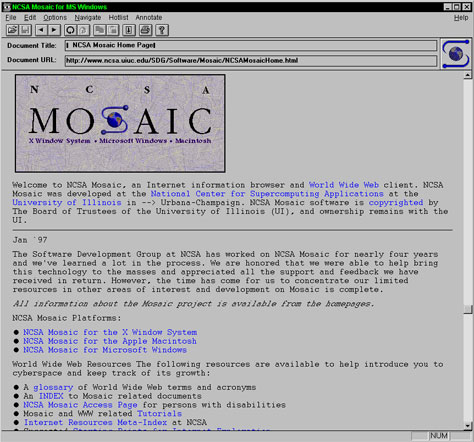
\includegraphics[width=130pt]{mosaic_browser.png}
  \end{figure}
\end{frame}

\begin{frame}{The beginning of the web}
  \begin{itemize}
    \item Plain text and images were the most advanced features
    \item In 1994, the World Wide Web Consortium (W3C) was founded
    \item Companies were able to contribute to the W3C specifications
    \item Today's web is a result of the ongoing efforts of an open web
  \end{itemize}
\end{frame}

\begin{frame}{The modern web}
  \begin{figure}[!htb]
    \centering
    
\includegraphics[width=270pt]{html5_phrase.png}
  \end{figure}
\end{frame}

\begin{frame}{Browser technologies}
  \begin{figure}[!htb]
    \centering
    
\includegraphics[width=270pt]{html5_css3_js.png}
  \end{figure}
\end{frame}

\begin{frame}{Browser architecture}
  \begin{figure}[!htb]
    \centering
    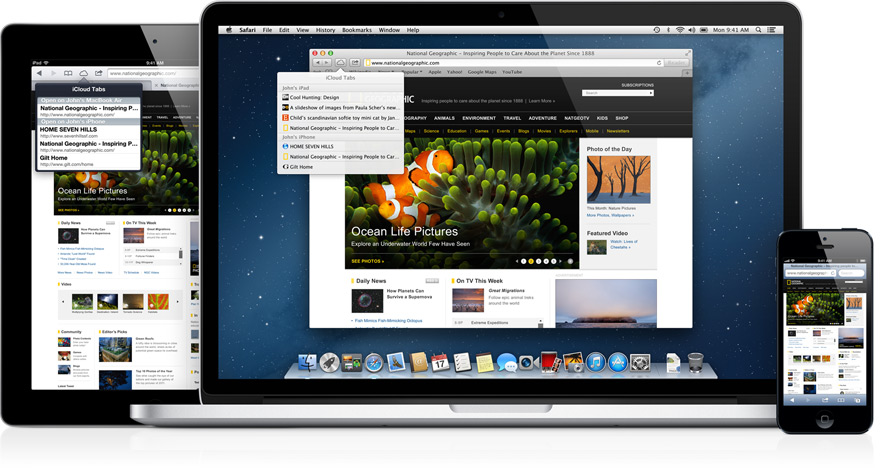
\includegraphics[width=220pt]{safari.png}
  \end{figure}
\end{frame}

\begin{frame}{Browser architecture}
  \begin{figure}[!htb]
    \centering
    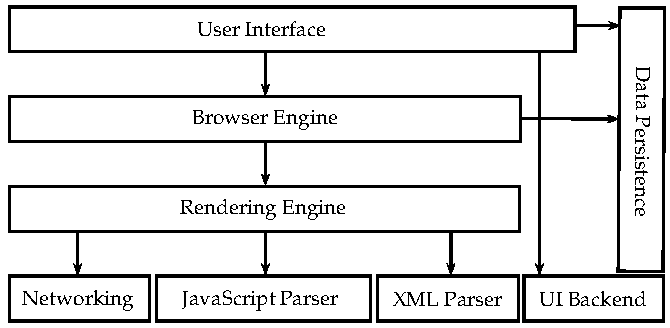
\includegraphics[width=220pt]{../chapters/basic_concepts/web_architecture.pdf}
  \end{figure}
\end{frame}

\subsection{Visual tracking}


\begin{frame}{Visual tracking}
  \begin{block}{}
      Tracking an object in a video sequence means continuously identifying its location when either the object or the camera are moving.
  \end{block}
  \begin{figure}[!htb]
    \centering
    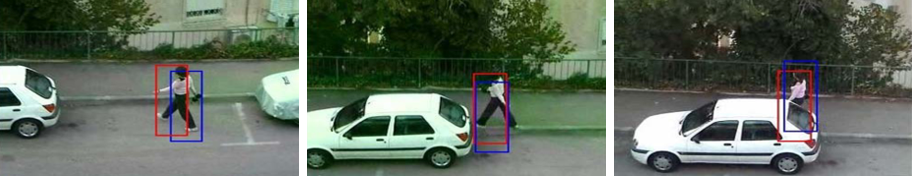
\includegraphics[width=\linewidth]{../chapters/basic_concepts/tracking_occlusion.png}
  \end{figure}
\end{frame}

\begin{frame}{Visual tracking}
  \begin{figure}[!htb]
    \centering
    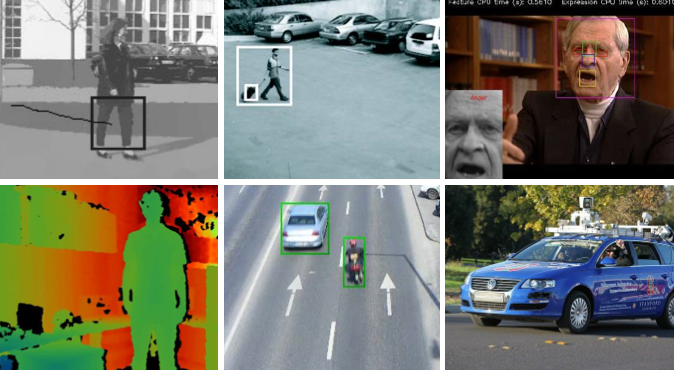
\includegraphics[width=200pt]{../chapters/basic_concepts/cv_applications.png}
  \end{figure}
\end{frame}

\subsection{Visual tracking on the web}

\begin{frame}{Visual tracking workflow on the web}
  \begin{figure}[!htb]
    \centering
    
\includegraphics[width=270pt]{workflow_off.png}
  \end{figure}
\end{frame}

\begin{frame}{1. Request user web-cam access}
  \begin{figure}[!htb]
    \centering
    
\includegraphics[width=270pt]{webrtc_confirmation.png}
  \end{figure}
\end{frame}

\begin{frame}{1. Request user web-cam access}
  \begin{figure}[!htb]
    \centering
    
\includegraphics[width=270pt]{workflow_1.png}
  \end{figure}
\end{frame}

\begin{frame}{2. Capture web-cam stream}
  \begin{figure}[!htb]
    \centering
    
\includegraphics[width=100pt]{webrtc.png}
  \end{figure}
\end{frame}

\begin{frame}[fragile]{2. Capture web-cam stream}
  \begin{lstlisting}[
                    language=C++,
                    label={lst:get_user_media1},
                    moredelim={**[is][\btHL<1>]{@1}{@}},
                    moredelim={**[is][{\btHL<2>}]{@2}{@}}
                  ]

  <script>
    navigator.@1getUserMedia@({ video: true }, function(localMediaStream) {
      // Stream captured
    }, onFail);
  </script>
  \end{lstlisting}
\end{frame}

\begin{frame}{2. Capture web-cam stream}
  \begin{figure}[!htb]
    \centering
    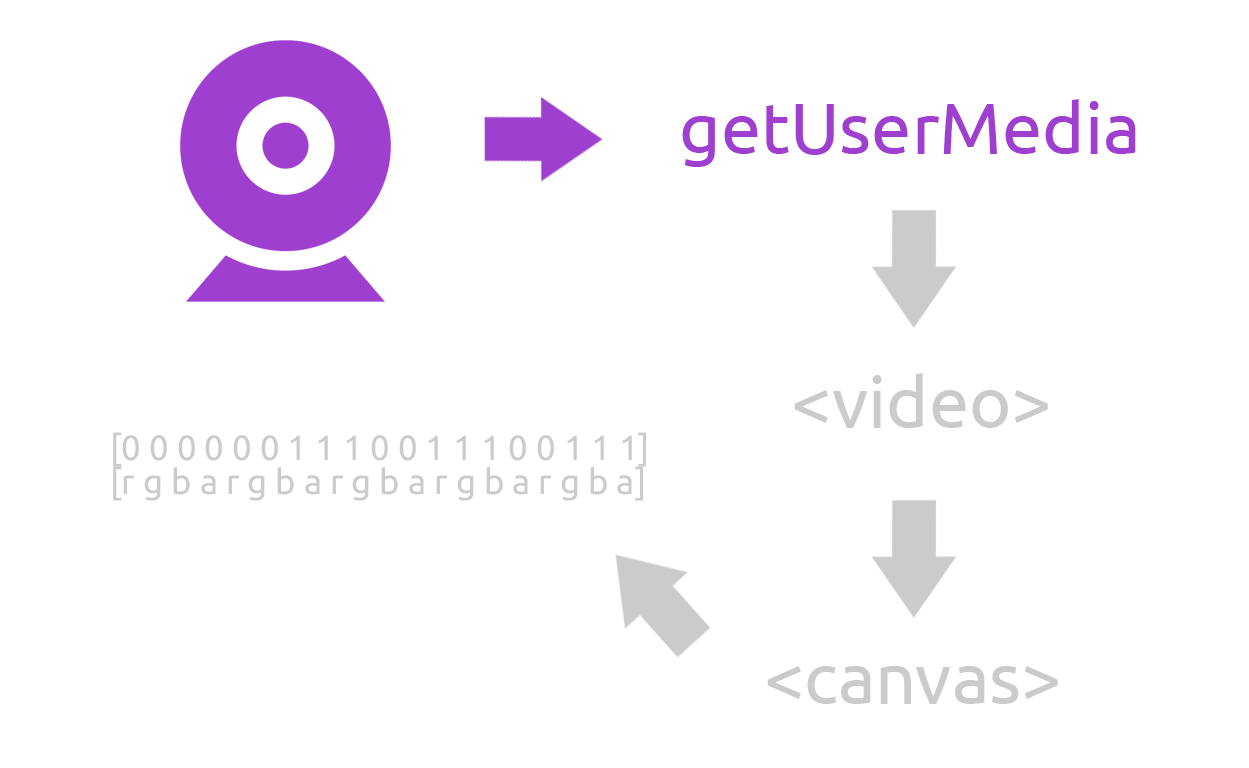
\includegraphics[width=270pt]{workflow_2.png}
  \end{figure}
\end{frame}

\begin{frame}{3. Reproduce web-cam stream into the video}
  \begin{figure}[!htb]
    \centering
    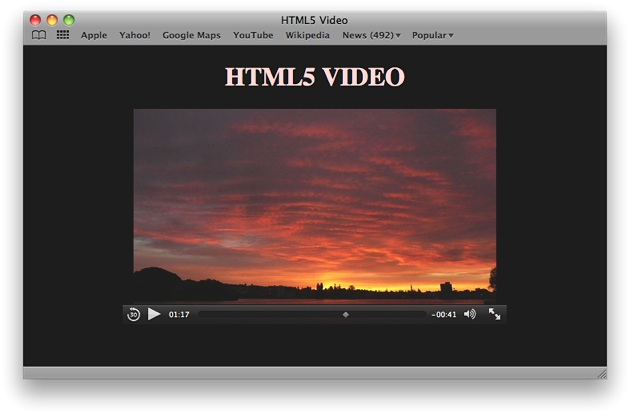
\includegraphics[width=220pt]{../chapters/basic_concepts/html5_audio_video.png}
  \end{figure}
\end{frame}

\begin{frame}[fragile]{3. Reproduce web-cam stream into the video}
  \begin{lstlisting}[
                    language=C++,
                    label={lst:get_user_media2},
                    moredelim={**[is][\btHL<1>]{@1}{@}},
                    moredelim={**[is][{\btHL<2>}]{@2}{@}},
                    moredelim={**[is][{\btHL<3>}]{@3}{@}}
                  ]

  @1<video autoplay></video>@
  <script>
    var video = document.querySelector('video');
    navigator.@2getUserMedia@({video: true}, function(localMediaStream) {
        @3video.src = window.URL.createObjectURL(localMediaStream);@
        video.onloadedmetadata = function(e) { alert('Ready to go.') };
    }, onFail);
  </script>
  \end{lstlisting}
\end{frame}

\begin{frame}{3. Reproduce web-cam stream into the video}
  \begin{figure}[!htb]
    \centering
    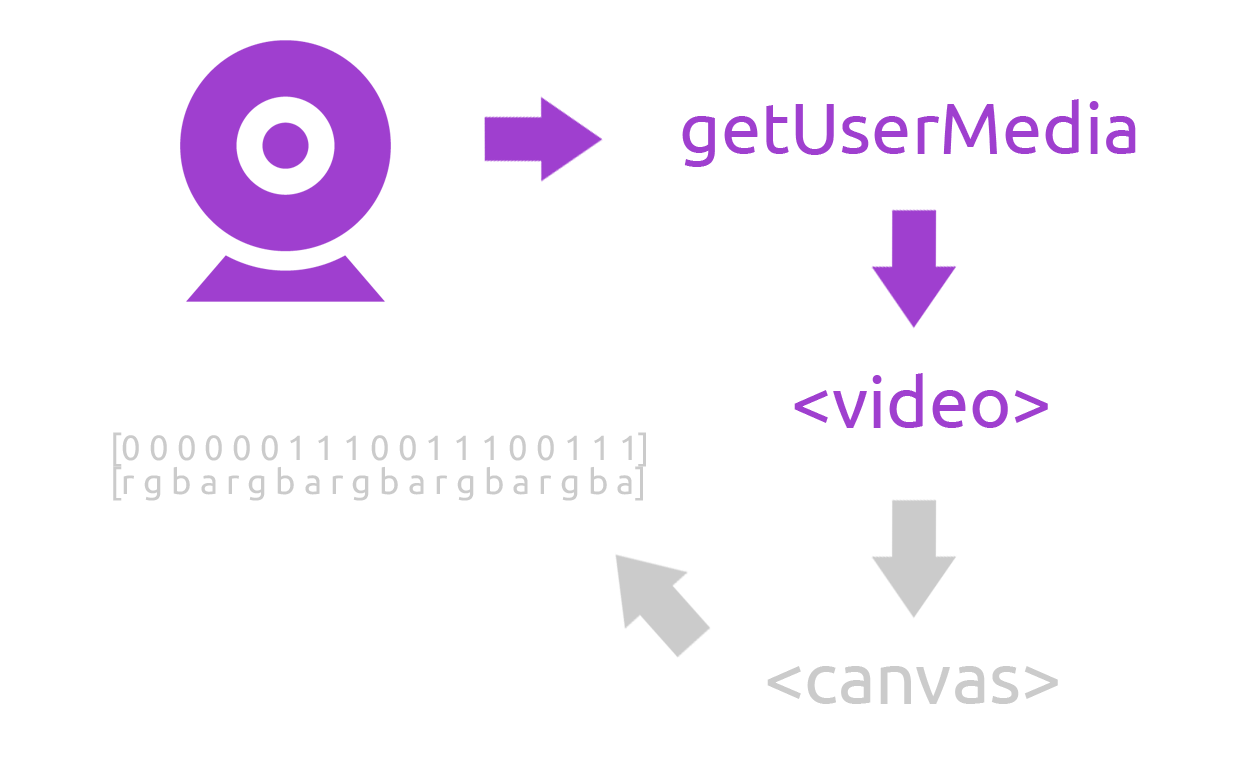
\includegraphics[width=270pt]{workflow_3.png}
  \end{figure}
\end{frame}

\begin{frame}{4. Process video data using canvas}
  \begin{figure}[!htb]
    \centering
    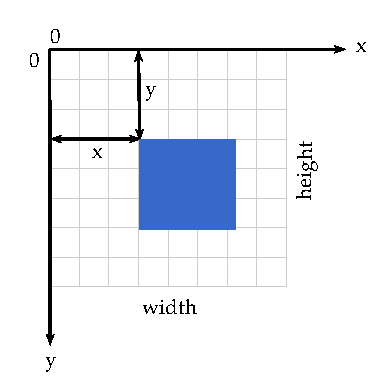
\includegraphics[width=130pt]{../chapters/basic_concepts/canvas_axis.pdf}
  \end{figure}
\end{frame}

\begin{frame}{4. Process video data using canvas}
  \begin{itemize}
    \item Introduced as a new element on HTML5
    \item Resolution-dependent bitmap canvas
    \item Two-dimensional grid, computer graphics coordinate system
    \item Can render images, video frames or shapes
  \end{itemize}
\end{frame}

\begin{frame}{4. Process video data using canvas}
  \begin{figure}[!htb]
    \centering
    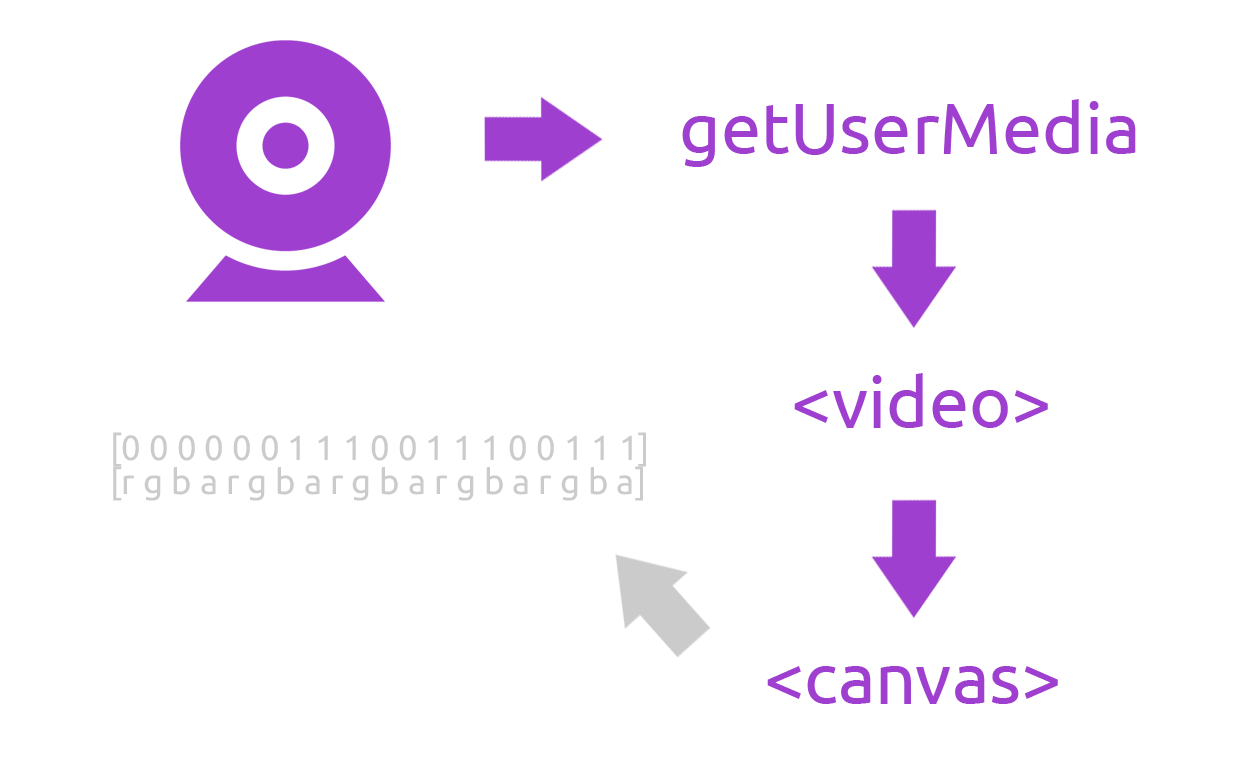
\includegraphics[width=270pt]{workflow_4.png}
  \end{figure}
\end{frame}

\begin{frame}{5. Access canvas data using JavaScript typed arrays}
  \begin{itemize}
    \item In the past, raw data was accessed as a string
    \item Browsers needed a quick way to manipulate raw binary data
    \item Typed data structures were added to JavaScript
    \item JavaScript-typed arrays access raw binary more efficiently
  \end{itemize}
\end{frame}

\begin{frame}{5. Access canvas data using JavaScript typed arrays}
  \begin{figure}[!htb]
    \begin{tikzpicture}[scale=0.8]
        \begin{axis}[
            bar width=15pt,
            enlarge x limits=0.25,
            height= 200pt,
            legend cell align=left,
            scaled y ticks=false,
            symbolic x coords={Firefox,Safari,Chrome},
            width=0.85*\textwidth,
            xmajorgrids=true,
            xtick=data,
            ybar=\pgflinewidth,
            ylabel={Operations per second (ops/sec)},
            ylabel style={yshift=10pt},
            ymajorgrids=true,
            ymin=0
        ]
            \addplot[style={wblue, fill=wblue}]
                coordinates {
                  (Firefox, 4437)
                  (Safari, 2607)
                  (Chrome, 679)
                };

            \addplot[style={wred, fill=wred}]
                coordinates {
                  (Firefox, 5841)
                  (Safari, 2797)
                  (Chrome, 1510)
                };

            \addplot[style={worange, fill=worange}]
                coordinates {
                  (Firefox, 7872)
                  (Safari, 3089)
                  (Chrome, 1510)
                };

            \legend{Array,Float32Array,Uint8Array}
        \end{axis}
    \end{tikzpicture}
  \end{figure}
\end{frame}

\begin{frame}{5. Access canvas data using JavaScript typed arrays}
  \begin{figure}[!htb]
    \centering
    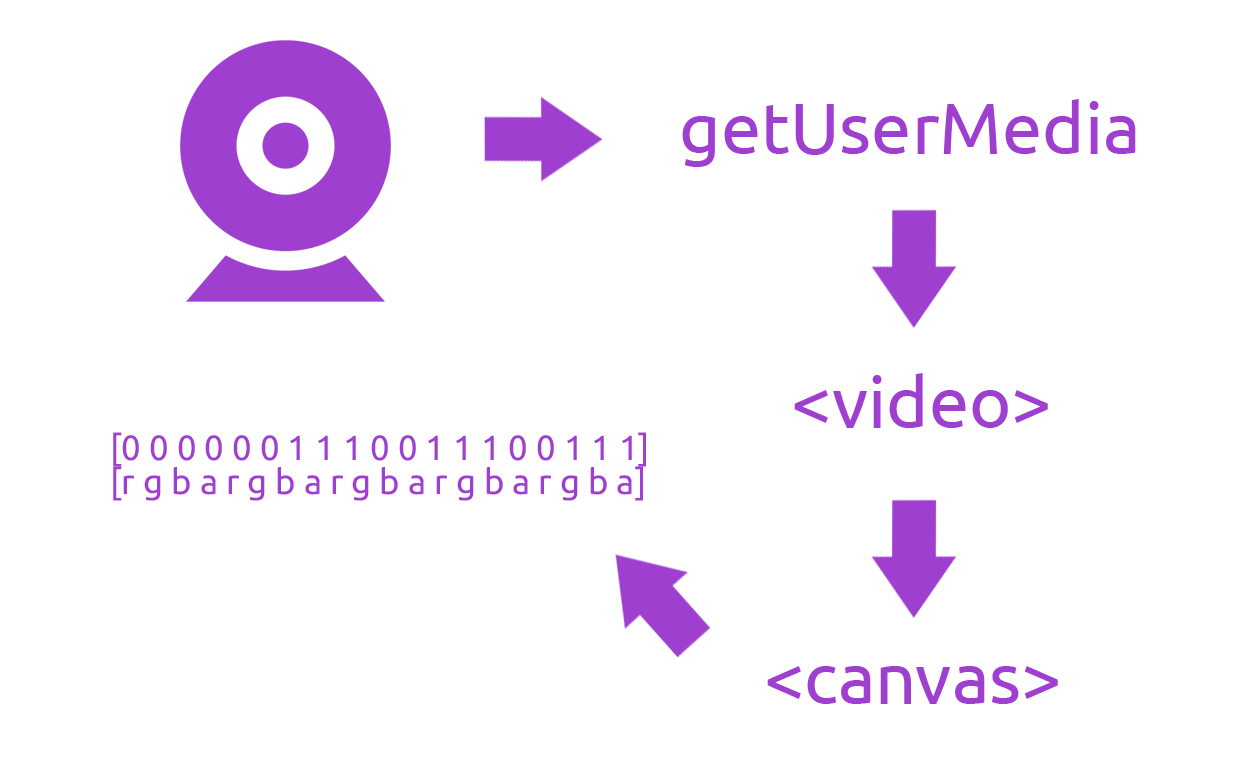
\includegraphics[width=270pt]{workflow_5.png}
  \end{figure}
\end{frame}

\begin{frame}{What is the relation between typed arrays and canvas?}
  \begin{itemize}
    \item Videos and images pixels can be drawn on a canvas bitmap
    \item Canvas raw binary data can be accessed from JavaScript
    \item Canvas array of pixels, is in row-major order
    \item Consider the $2\times3$ array $\begin{bmatrix}
1 & 2 & 3\\
4 & 5 & 6
\end{bmatrix}$, in row-major order it is laid out contiguously in linear memory as $\begin{bmatrix}
1 & 2 & 3 & 4 & 5 & 6
\end{bmatrix}$.
  \end{itemize}
\end{frame}

\begin{frame}{What is the relation between typed arrays and canvas?}
  \begin{figure}[!htb]
    \centering
    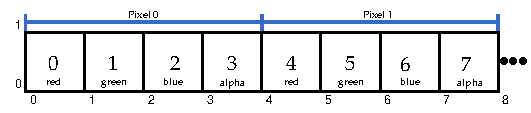
\includegraphics[width=\linewidth]{../chapters/basic_concepts/imagedata_array.pdf}
  \end{figure}
\end{frame}
% % -----------------------------------------------------------------------------
\section{Tracking library for the web}

\begin{frame}{Related work}
  \begin{itemize}
    \item FLARToolKit: a port of ARToolKit marker tracking library to ActionScript
  \end{itemize}
  \begin{figure}[!htb]
    \centering
    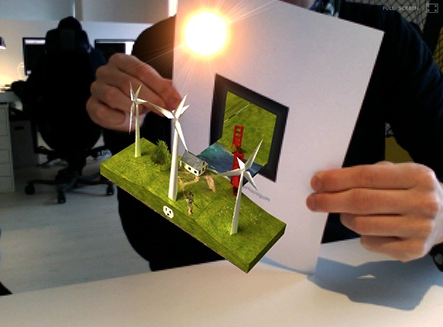
\includegraphics[width=130pt]{../chapters/tracking_library_for_the_web/flartoolkit.png}
  \end{figure}
\end{frame}

\begin{frame}{Related work}
  \begin{itemize}
    \item JSARToolkit: is a JavaScript port of FLARToolKit
  \end{itemize}
  \begin{figure}[!htb]
    \centering
    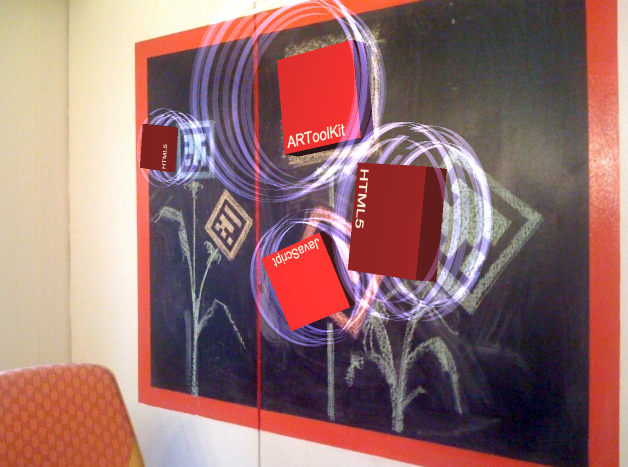
\includegraphics[width=130pt]{../chapters/tracking_library_for_the_web/jsartoolkit.png}
  \end{figure}
\end{frame}

\begin{frame}{Related work}
  \begin{itemize}
    \item Unifeye Viewer: a robust markerless tracking solution for the web to ActionScript
  \end{itemize}
  \begin{figure}[!htb]
    \centering
    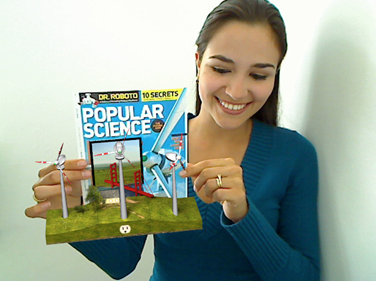
\includegraphics[width=130pt]{../chapters/tracking_library_for_the_web/unifeyeviewer.png}
  \end{figure}
\end{frame}

\begin{frame}{Flash vs HTML5}
  \begin{figure}[!htb]
    \centering
    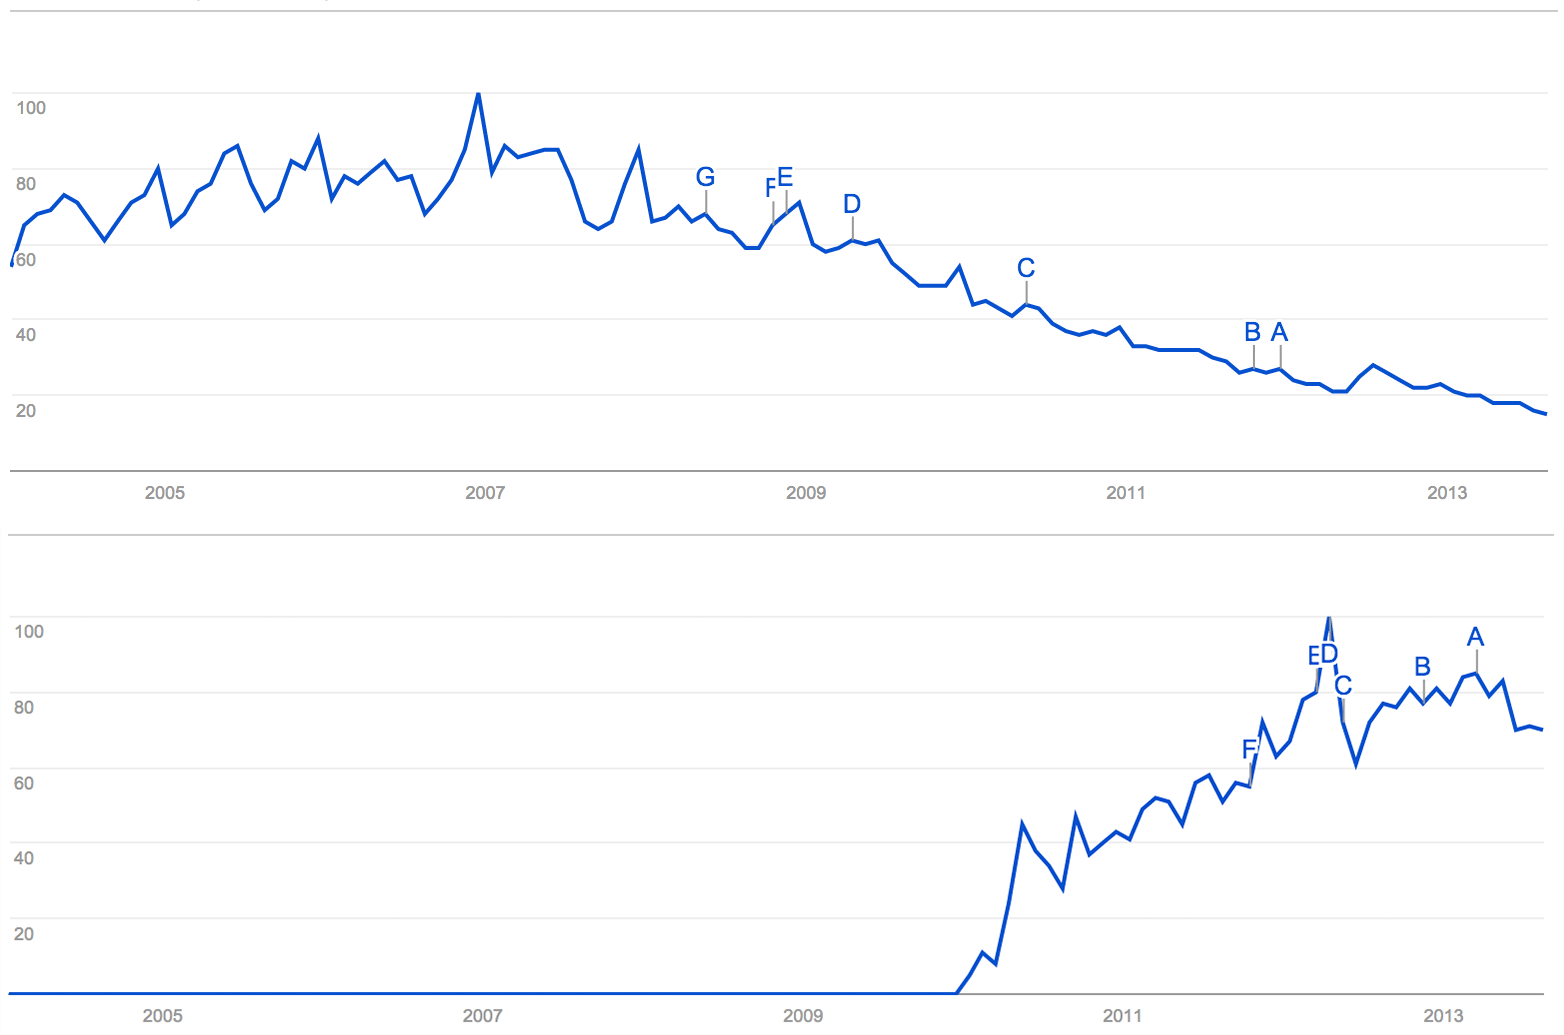
\includegraphics[width=220pt]{trend.png}
  \end{figure}
\end{frame}

\begin{frame}{tracking.js}
  \begin{figure}[!htb]
    \centering
    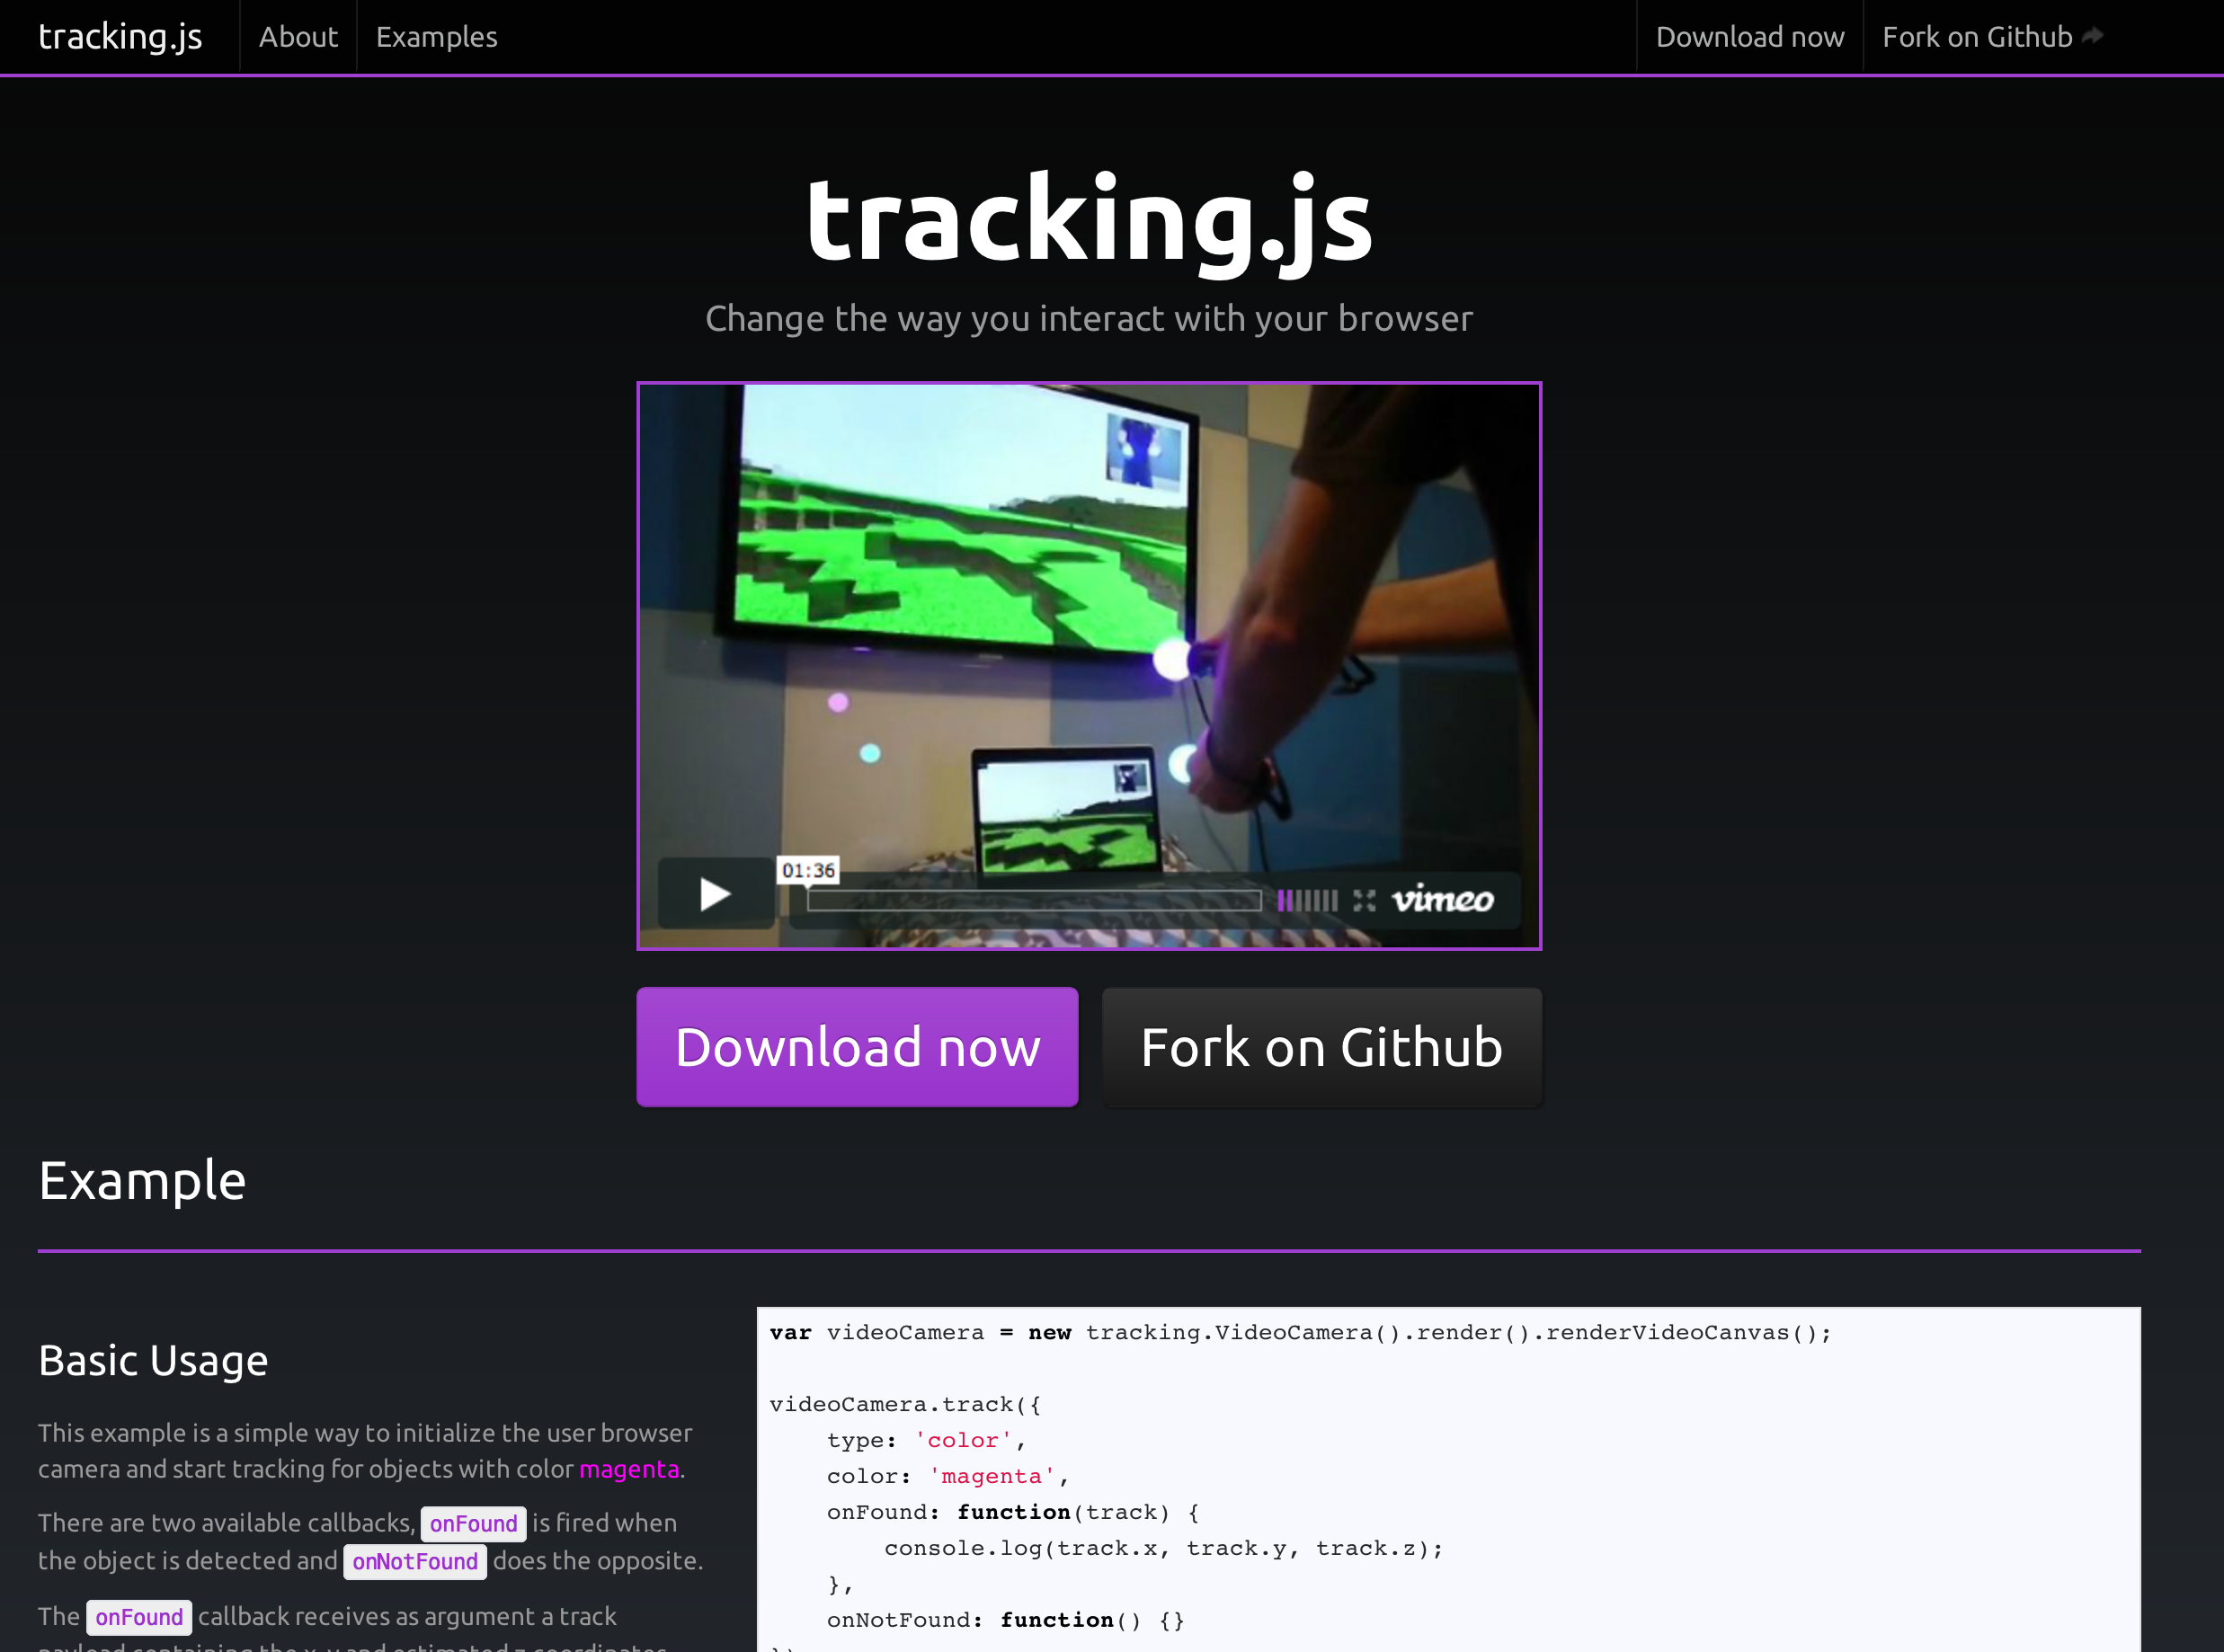
\includegraphics[width=180pt]{site.png}
  \end{figure}
\end{frame}

\begin{frame}{tracking.js}
  \begin{block}{Tracking library for the web}{
    Common infrastructure to develop visual tracking applications and to accelerate the use of those techniques on the web in commercial products.
  }
  \end{block}
\end{frame}

\begin{frame}{Library features}
  \begin{block}{1. Color tracking}
    \begin{figure}[!htb]
      \centering
      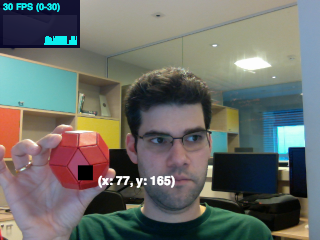
\includegraphics[width=120pt]{../chapters/evaluation/color_object_3.png}
    \end{figure}
  \end{block}
\end{frame}

\begin{frame}{Library features}
  \begin{block}{2. Rapid object detection (Viola Jones)}
    \begin{figure}[!htb]
      \centering
      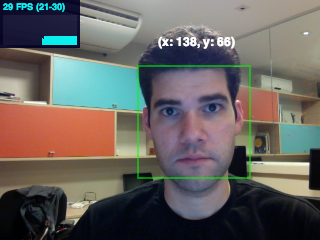
\includegraphics[width=120pt]{../chapters/evaluation/viola_face.png}
    \end{figure}
  \end{block}
\end{frame}

\begin{frame}{Library features}
  \begin{block}{3. Markerless tracking algorithm}
    \begin{figure}[!htb]
      \centering
      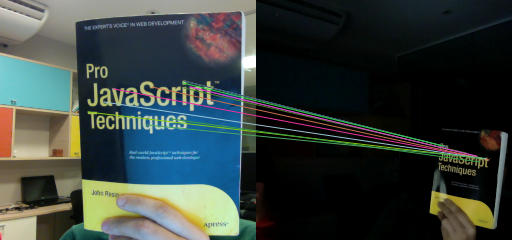
\includegraphics[width=200pt]{../chapters/evaluation/keypoints_brief.png}
    \end{figure}
  \end{block}
\end{frame}

\begin{frame}{Library modules - Base classes}
  \begin{figure}[!htb]
      \tikzumlset{font=\tiny}
      \begin{tikzpicture}
          \umlclass[x=100pt]{Math}{}

          \umlclass{Attribute}{}

          \umlclass[y=-50pt]{DOMElement}{}

          \umlclass[y=-85pt,x=-80pt]{Canvas}{}

          \umlclass[y=-110pt]{Video}{}

          \umlclass[y=-110pt,x=100pt]{VideoCamera}{}

          \umlinherit[geometry=-|]{DOMElement}{Attribute}
          \umlinherit[geometry=-|]{Canvas}{DOMElement}
          \umlinherit[geometry=-|]{Video}{DOMElement}
          \umlinherit[geometry=|-]{VideoCamera}{Video}
      \end{tikzpicture}
  \end{figure}
\end{frame}

\begin{frame}{Library modules - Visual tracking classes}
  \begin{figure}[!htb]
      \tikzumlset{font=\tiny}
      \begin{tikzpicture}
          \umlclass{FAST}{}{
            findCorners(data, threshold) : Array\\
          }

          \umlclass[y=-55pt]{BRIEF}{}{
            getDescriptors(data, corners) : Array\\
            match(c1, d1, c2, d2) : Array\\
          }

          \umlclass[y=-110pt]{ViolaJones}{}{
            find() : Array\\
            evalStage() : boolean\\
          }

          \umlclass[y=-110pt,x=140pt]{Color}{}{
            find() : Array\\
          }

          \umlclass[x=140pt]{RANSAC}{}{
            find(matches) : void\\
            score() : Number\\
          }

          \umlclass[y=-55pt,x=140pt]{Homography}{}{
              score(H, matches) : Number\\
          }

          \umlinherit[geometry=-|]{Homography}{RANSAC}
      \end{tikzpicture}
  \end{figure}
\end{frame}

\begin{frame}{Color tracking algorithm}
  \begin{figure}[!htb]
    \centering
    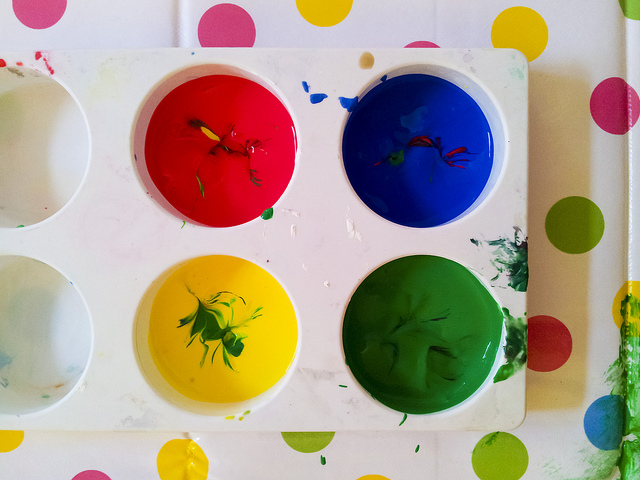
\includegraphics[width=170pt]{color_blob.png}
    \caption{\copyright\ \url{http://www.flickr.com/photos/laynecom/8674644879/}}
  \end{figure}
\end{frame}

\begin{frame}[fragile]{Color tracking algorithm}
  \begin{lstlisting}[language=C++]
    var videoCamera = new tracking.VideoCamera();
    videoCamera.track({
        type: 'color',
        color: 'magenta',
        onFound: function(track) {
          // do your logic here.
        }
    });
  \end{lstlisting}
\end{frame}

\begin{frame}{Color tracking algorithm - Color difference evaluation}
  $$\|C_1-C_2\|=\sqrt{(C_{1,R}-C_{2,R})^2 + (C_{1,G}-C_{2,G})^2 + (C_{1,B}-C_{2,B})^2}$$

  \begin{figure}[!htb]
    \centering
    \begin{tikzpicture}[scale = 0.5]
      \def \radi{3}
      \def \x{3}
      \def \y{3}
      \def \z{3}

      \begin{scope}
       \begin{scope}[color=gray, thin]
        \foreach \xi in {0,...,\radi}{ \draw (\xi,\radi,0) -- (\xi,0,0) -- (\xi,0,\radi); }%
        \foreach \yi in {1,...,\radi}{ \draw (0,\yi,\radi) -- (0,\yi,0) -- (\radi,\yi,0); }%
        \foreach \zi in {0,...,\radi}{ \draw (0,\radi,\zi) -- (0,0,\zi) -- (\radi,0,\zi); }%
       \end{scope}

       \draw[-latex, thick, color=black] (0,0,0) -- (4,0,0) node[anchor=west] {R};%
       \draw[-latex, thick, color=black] (0,0,0) -- (0,4,0) node[anchor=east] {B};%
       \draw[-latex, thick, color=black] (0,0,0) -- (0,0,4) node[anchor=east] {G};%

       \draw[color=black, ultra thick]
       (0,\y,\z) -- (\x,\y,\z) -- (\x,\y,0) (\x,\y,\z) -- (\x,0,\z);
      \end{scope}

      \draw (-1,0) arc (180:360:1cm and 0.5cm);
      \draw[dashed] (-1,0) arc (180:0:1cm and 0.5cm);
      \draw (0,1) arc (90:270:0.5cm and 1cm);
      \draw[dashed] (0,1) arc (90:-90:0.5cm and 1cm);
      \draw (0,0) circle (1cm);
      \shade[ball color=gray,opacity=1] (0,0) circle (0.1cm);
     \end{tikzpicture}
  \end{figure}
\end{frame}

\begin{frame}{Color tracking algorithm - Color blob detection}
  \begin{figure}[!htb]
    \centering
    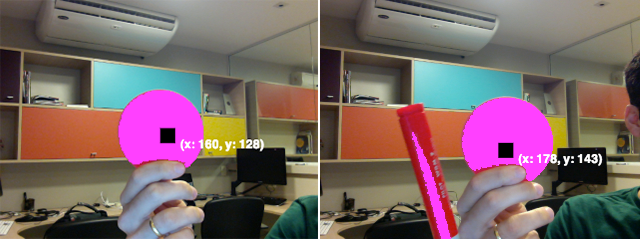
\includegraphics[width=260pt]{../chapters/tracking_library_for_the_web/color_tracking.png}
  \end{figure}
\end{frame}

\begin{frame}{Rapid object detection (Viola Jones)}
  \begin{figure}[!htb]
    \centering
    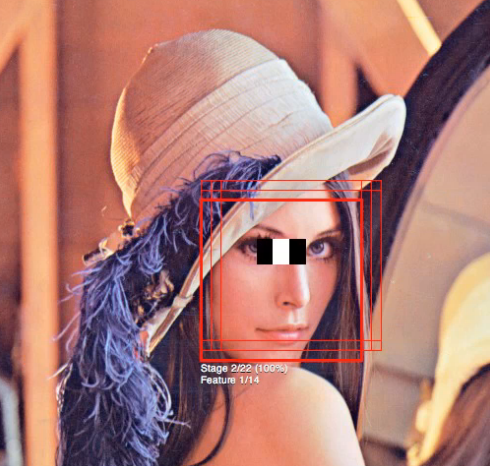
\includegraphics[width=140pt]{viola.png}
  \end{figure}
\end{frame}

\begin{frame}[fragile]{Rapid object detection (Viola Jones)}
  \begin{lstlisting}[language=C++]
    var videoCamera = new tracking.VideoCamera();
    videoCamera.track({
        type: 'human',
        data: 'frontal_face',
        onFound: function(track) {
          // do your logic here.
        }
    });
  \end{lstlisting}
\end{frame}

\begin{frame}{Rapid object detection (Viola Jones)}
  \begin{itemize}
    \item Robust and extremely rapid object detection
    \item Became popular mainly because rapid face detection
    \item A training phase is required
    \item A scanning detector is what makes the detection
  \end{itemize}
\end{frame}

\begin{frame}{Rapid object detection (Viola Jones)}
  \begin{figure}[!htb]
    \centering
    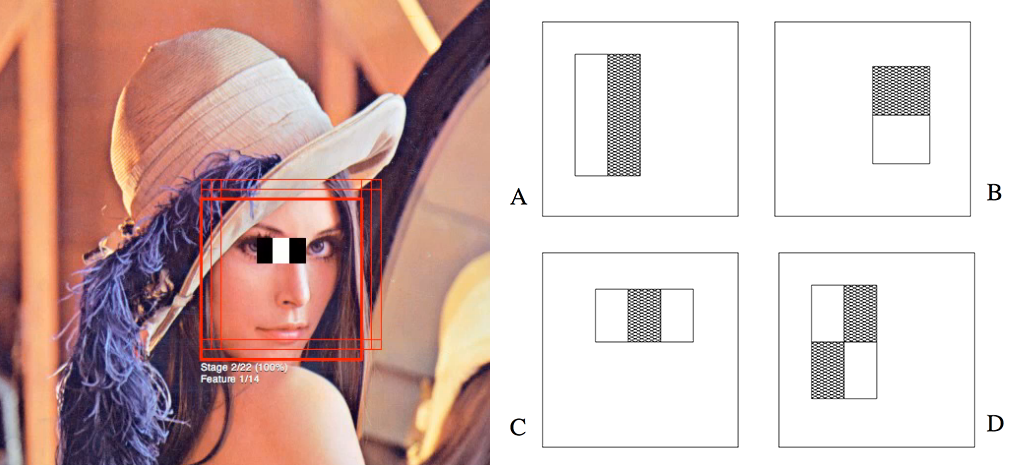
\includegraphics[width=220pt]{features_viola.png}
  \end{figure}
\end{frame}

\begin{frame}{Rapid object detection (Viola Jones)}
  \begin{block}{Integral Image}
      Rectangle features can be computed very rapidly using an intermediate representation for the image which we call the integral image.
  \end{block}
  The integral image at location $x, y$ contains the sum of the pixels above and to the left of $x, y$, inclusive
  $$ii(x,y)=\sum_{x'\leq x,y'\leq y}{i(x',y')}$$
\end{frame}

\begin{frame}{Rapid object detection (Viola Jones)}
  \begin{figure}[!htb]
    \centering
    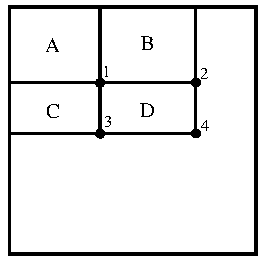
\includegraphics[width=100pt]{integral_image.pdf}
  \end{figure}
\end{frame}

\begin{frame}{Rapid object detection (Viola Jones)}
  \begin{block}{Scanning detector algorithm}
      \begin{enumerate}
        \item Create or scale a $20\times20$ squared block by $1.25$ per iteration
        \item Loop the block by $\Delta$ pixels over the image
        \item For each block location, loop the tree and evaluate each stage
        \item Positive stage evaluate next stage, otherwise stops the loop
        \item If all stages were positive store the rectangle
        \item Once the tree is done, group the overlapping rectangles
        \item Find the best rectangle of each the group (merging phase)
      \end{enumerate}
  \end{block}
\end{frame}

\begin{frame}{Rapid object detection (Viola Jones)}
  \begin{block}{Optimized merging phase}
      Rectangles are used partitioned into a disjoint set data structure. On this work it was replaced by an alternative called Minimum Neighbor Area Grouping.
  \end{block}
  \begin{block}{Minimum Neighbor Area Grouping}
      Simple loop trough the possible rectangles comparing the current rectangle with all other not yet compared. If their area overlaps by $\eta=0.5$ the smallest rectangle of the set is selected.
  \end{block}
\end{frame}

\begin{frame}{Feature detector (FAST)}
  \begin{figure}[!htb]
    \centering
    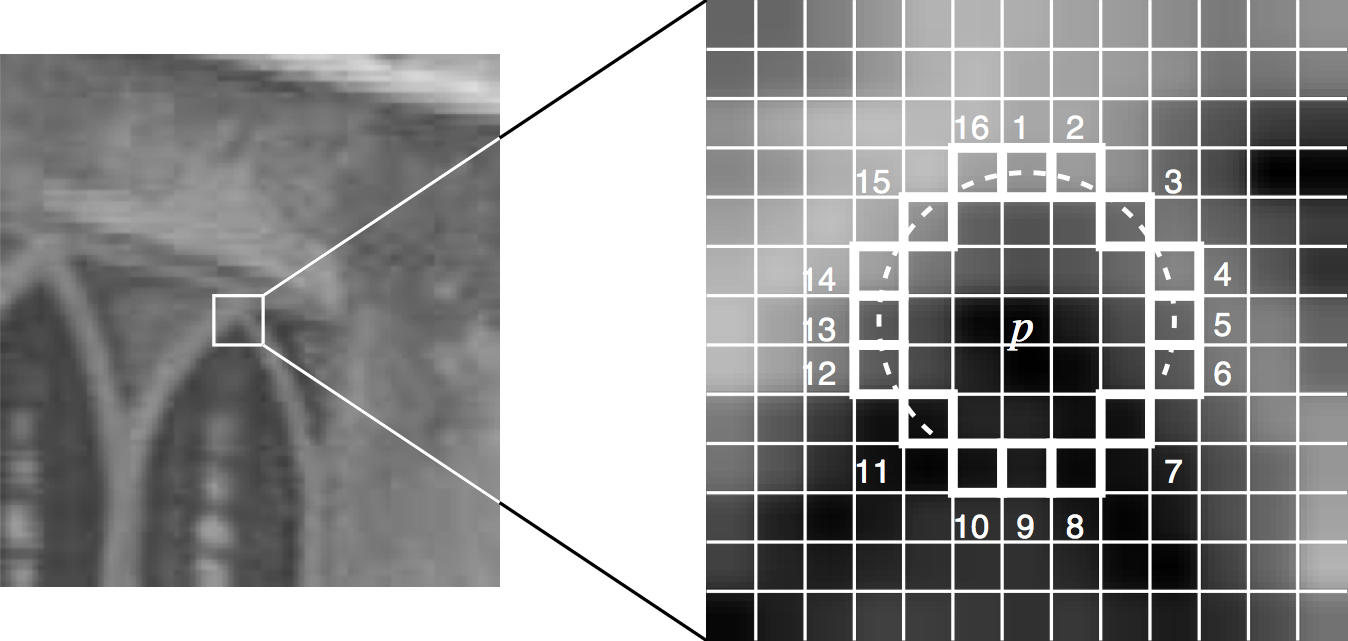
\includegraphics[width=220pt]{../chapters/tracking_library_for_the_web/fast.png}
  \end{figure}
\end{frame}

\begin{frame}{Feature detector (FAST)}
  \begin{figure}[!htb]
    \centering
    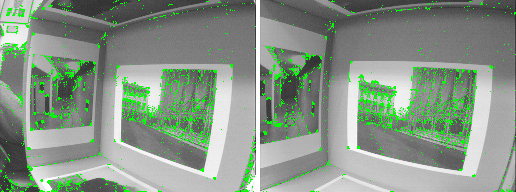
\includegraphics[width=290pt]{../chapters/tracking_library_for_the_web/keypoints.png}
  \end{figure}
\end{frame}

\begin{frame}{Feature extractor (BRIEF)}
  \begin{figure}[!htb]
    \centering
    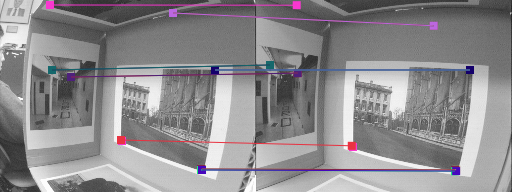
\includegraphics[width=290pt]{../chapters/evaluation/keypoints_building.png}
  \end{figure}
\end{frame}

\begin{frame}{Feature extractor (BRIEF)}
  To generate the binary strings it is defined the test $\tau$ on patch \textbf{p} of size \textbf{S $\times$ S} as:

  $$\tau(\textbf{p}; x, y) :=
  \begin{cases}
    1 &\mbox{if}\quad \textbf{p(x)} < \textbf{p(y)},\\
    0 &\mbox{otherwise}
  \end{cases}$$
\end{frame}

\begin{frame}{Feature extractor (BRIEF)}
  The $n_{d}$-dimensional bit-string is our BRIEF descriptor for each keypoint:

  $$f_{n_{d}}(\textbf{p}) := \sum_{1 \le i \le n_{d}} 2^{i-1} \tau(\textbf{p}; x, y).$$

  In this work $n_{d}= 128$ was used. The number of bytes required to store the descriptor can be calculated by $k = n_{d}/8$.
\end{frame}

\begin{frame}{Feature extractor (BRIEF)}
  \begin{figure}[!htb]
    \centering
    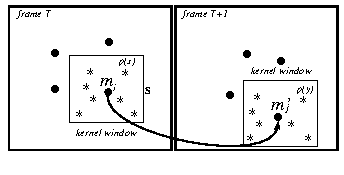
\includegraphics[width=220pt]{../chapters/tracking_library_for_the_web/BRIEF.pdf}
  \end{figure}
\end{frame}

\begin{frame}{Feature extractor (BRIEF)}
  The weighted Hamming distance is computed by:
  $$WHam(x, y)=\sum_{i=1}^{n}w_i(b_i(x)\otimes b_i(y))$$
  $$b_1=0000000001...$$
  $$b_2=0000000011...$$
  $$b_1 \otimes b_2=0000000010...$$
  $$WHam=1$$
\end{frame}

\begin{frame}{Feature extractor (BRIEF)}
  \begin{figure}[!htb]
    \centering
    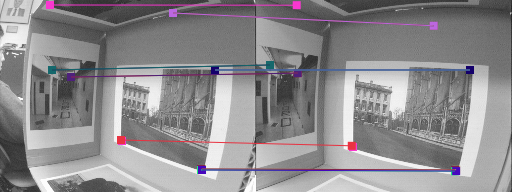
\includegraphics[width=290pt]{../chapters/evaluation/keypoints_building.png}
  \end{figure}
\end{frame}

\begin{frame}{Homography estimation}
  \begin{figure}[!htb]
    \centering
    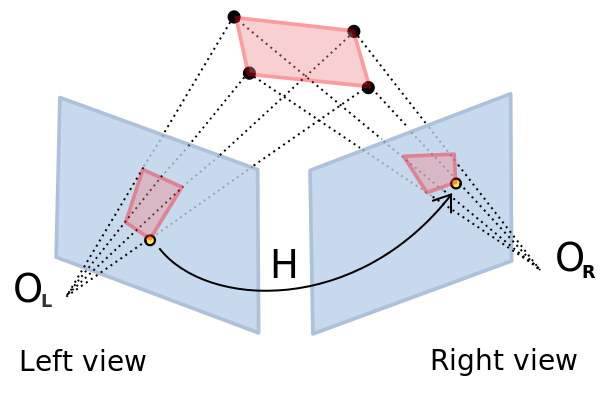
\includegraphics[width=160pt]{homography.png}
  \end{figure}
\end{frame}

\begin{frame}{Random sample consensus (RANSAC)}
  \begin{block}{}
      RANSAC (Random Sample Consensus) is an iterative method to estimate parameters of a mathematical model from a set of observed data which contains outliers. It is the most commonly used robust estimation method for homographies.
  \end{block}
\end{frame}
% % -----------------------------------------------------------------------------
\section{Results and evaluation}

\begin{frame}{Evaluation methodology}
  \begin{block}{1. Examples}
  \end{block}

  \begin{block}{2. Performance}
  Frames per second (FPS) metric. All tests were executed on Google Chrome browser version 28.0.1500.71, Mac OS X 10.8.3, 2.6 GHz Intel Core i7 16 GB 1600 MHz RAM.
  \end{block}

  \begin{block}{3. Partial occlusion robustness}
  Examples of how each technique behaves under partial occlusion.
  \end{block}
\end{frame}

\begin{frame}{Evaluation methodology}
  \begin{figure}[!htb]
    \centering
    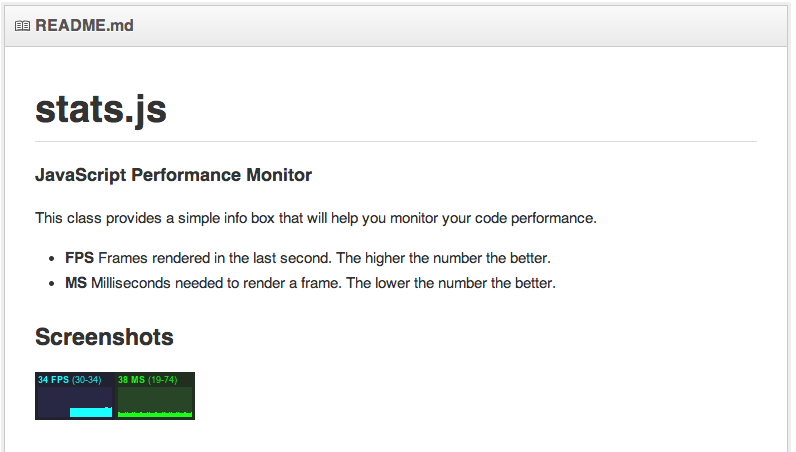
\includegraphics[width=260pt]{statsjs.png}
  \end{figure}
\end{frame}

\subsection{Color tracking algorithm}

\begin{frame}{Examples}
  \begin{figure}[!htb]
    \centering
    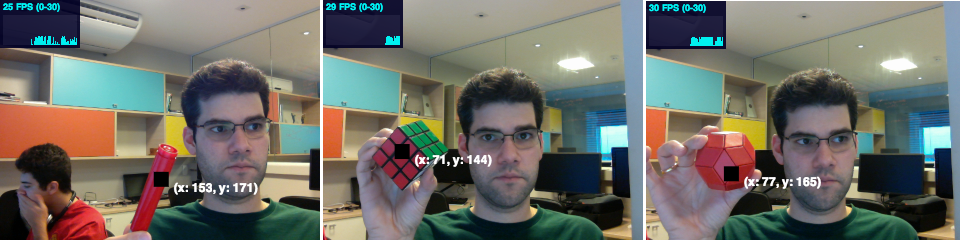
\includegraphics[width=\linewidth]{../chapters/evaluation/color_object.png}
  \end{figure}
\end{frame}

\begin{frame}{Performance}
  \begin{figure}[!htb]
    \centering
      \begin{tikzpicture}[scale = 0.8]
      \begin{axis}[
          enlarge x limits=0.03,
          minor tick num=1,
          xlabel=Number of pixels detected,
          ylabel=Frames per second (FPS)]

          \addplot[wblue,mark=x] coordinates {
          (174,30)
          (178,30)
          (178,30)
          (172,30)
          (164,30)
          (164,30)
          (150,30)
          (150,30)
          (156,30)
          (192,30)
          (192,30)
          (200,30)
          (200,30)
          (184,30)
          (160,30)
          (160,30)
          (160,30)
          (160,30)
          (158,30)
          (158,30)
          (162,30)
          (162,30)
          (180,30)
          (160,30)
          (160,30)
          (154,30)
          (154,30)
          (162,30)
          (162,30)
          (194,30)
          (194,29)
          (172,29)
          (172,29)
          (182,29)
          (134,29)
          (134,29)
          (160,29)
          (160,29)
          (176,29)
          (176,29)
          (154,29)
          (154,29)
          (184,29)
          (184,29)
          (172,29)
          (182,29)
          (182,29)
          (164,29)
          (164,29)
          (148,29)
          (148,29)
          (122,29)
          (122,29)
          (122,29)
          (138,29)
          (138,29)
          (162,29)
          (162,29)
          (176,29)
          (176,29)
          (208,30)
          (208,30)
          (208,30)
          (208,30)
          (200,30)
          (202,30)
          (202,30)
          (194,30)
          (194,30)
          (198,30)
          (198,30)
          (246,30)
          (246,30)
          (308,30)
          (308,30)
          (274,30)
          (254,30)
          (254,30)
          (322,30)
          (322,30)
          (406,30)
          (406,30)
          (434,30)
          (434,30)
          (408,30)
          (412,30)
          (470,30)
          (478,30)
          (478,30)
          (478,30)
          (546,29)
          (668,29)
          (668,29)
          (660,29)
          (700,29)
          (700,29)
          (756,29)
          (756,29)
          (848,29)
          (848,29)
          (890,29)
          (890,29)
          (884,29)
          (884,29)
          (880,29)
          (914,29)
          (914,29)
          (910,29)
          (910,29)
          (934,29)
          (934,29)
          (908,29)
          (908,29)
          (898,29)
          (974,29)
          (974,29)
          (998,29)
          (998,29)
          (1016,29)
          (1016,29)
          (1100,30)
          (1100,30)
          (1044,30)
          (1044,30)
          (1090,30)
          (1074,30)
          (1074,30)
          (1160,30)
          (1160,30)
          (1170,30)
          (1170,30)
          (1222,30)
          (1222,30)
          (1160,30)
          (1160,30)
          (1216,30)
          (1170,30)
          (1170,30)
          (1108,30)
          (1108,30)
          (1110,30)
          (1110,30)
          (1148,30)
          (1148,30)
          (1158,30)
          (1140,30)
          (1140,30)
          (1202,30)
          (1232,30)
          (1232,29)
          (1342,29)
          (1342,29)
          (1362,29)
          (1472,29)
          (1548,29)
          (1638,29)
          (1638,29)
          (1762,29)
          (1822,29)
          (1822,29)
          (1814,29)
          (1850,29)
          (1880,29)
          (1880,29)
          (1856,29)
          (1854,29)
          (1854,29)
          (1974,29)
          (1980,29)
          (1992,29)
          (2076,29)
          (2138,29)
          (2138,23)
          (2202,23)
          (2288,23)
          (2288,23)
          (2366,23)
          (2366,23)
          (2386,23)
          (2432,23)
          (2466,23)
          (2466,23)
          (2548,23)
          (2632,23)
          (2632,23)
          (2692,23)
          (2738,23)
          (2742,23)
          (2742,23)
          (2854,23)
          (2812,23)
          (2812,23)
          (2852,19)
          (2856,19)
          (2914,19)
          (2914,19)
          (2974,19)
          (2974,19)
          (2976,19)
          (3042,19)
          (3026,19)
          (3080,19)
          (3090,19)
          (3146,19)
          (3130,19)
          (3142,19)
          (3142,19)
          (3156,19)
          (3186,19)
          (3198,19)
          (3208,19)
          (3218,18)
          (3220,18)
          (3220,18)
          (3286,18)
          (3316,18)
          (3376,18)
          (3370,18)
          (3392,18)
          (3404,18)
          (3408,18)
          (3442,18)
          (3450,18)
          (3492,18)
          (3516,18)
          (3518,18)
          (3516,18)
          (3512,15)
          (3502,15)
          (3524,15)
          (3546,15)
          (3550,15)
          (3560,15)
          (3586,15)
          (3616,15)
          (3654,15)
          (3692,15)
          (3692,15)
          (3718,15)
          (3766,15)
          (3820,15)
          (3824,15)
          (3852,15)
          (3894,15)
          (3948,15)
          (3988,15)
          (4024,15)
          (4068,15)
          (4150,15)
          (4314,15)
          (4500,15)
          (4612,15)
          (4670,15)
          (4784,15)
          (4894,15)
          (4912,15)
          (4920,13)
          (4994,13)
          (5062,13)
          (5160,13)
          (5218,13)
          (5230,13)
          (5378,13)
          (5404,13)
          (5494,13)
          (5590,13)
          (5626,13)
          (5734,11)
          (5816,11)
          (5942,11)
          (6108,11)
          (6278,11)
          (6370,11)
          (6450,11)
          (6528,11)
          (6770,11)
          (6806,9)
          (7040,9)
          (7246,9)
          (7448,9)
          (7698,9)
          (7788,9)
          (7846,9)
          (7882,7)
          (7940,7)
          (7996,7)
          (8012,7)
          (7966,7)
          (7412,7)
           };

           \draw [red] ({rel axis cs:0,0}|-{axis cs:15,25}) -- ({rel axis cs:1,0}|-{axis cs:15,25}) node [pos=0.0, above] {};
      \end{axis}
      \end{tikzpicture}
  \end{figure}
\end{frame}

\begin{frame}{Oclusion robustness}
  \begin{figure}[!htb]
    \centering
    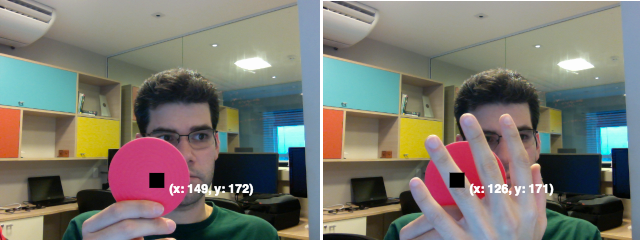
\includegraphics[width=220pt]{../chapters/evaluation/color_occlusion.png}
  \end{figure}
\end{frame}

\subsection{Rapid object detection (Viola Jones)}

\begin{frame}{Examples}
  \begin{figure}[!htb]
    \centering
    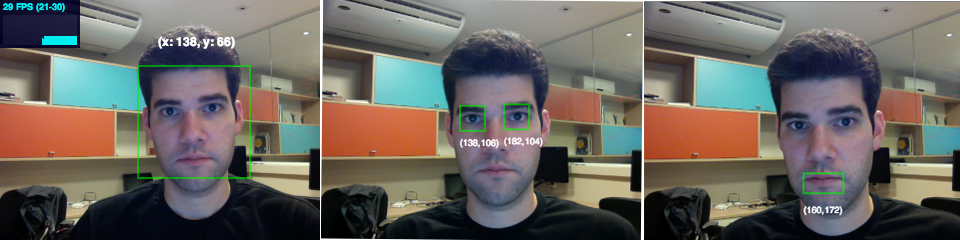
\includegraphics[width=\linewidth]{../chapters/evaluation/viola_overview.png}
  \end{figure}
\end{frame}

\begin{frame}{Examples}
  \begin{figure}[!htb]
    \centering
    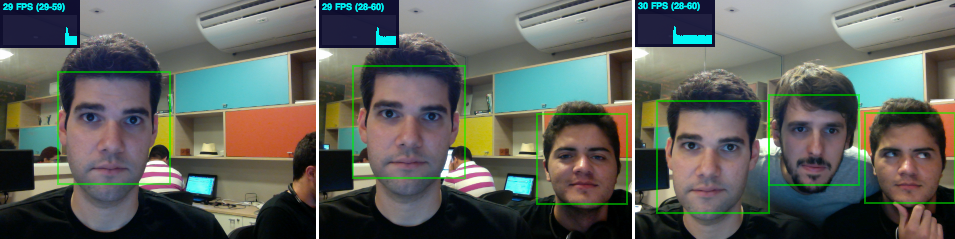
\includegraphics[width=\linewidth]{../chapters/evaluation/viola.png}
  \end{figure}
\end{frame}

\begin{frame}{Performance}
  \begin{figure}[!htb]
    \centering
      \begin{tikzpicture}[scale = 0.8]
      \begin{axis}[
          enlarge x limits=0.03,
          minor tick num=1,
          xlabel=Number of detected faces,
          ylabel=Frames per second (FPS)]

          \addplot[wblue,mark=x] coordinates {
               (1,30)
               (2,29)
               (3,30)
               (4,27)
               (5,25)
               (6,20)
               (7,17)
               (8,16)
               (9,16)
               (10,15)
               (11,15)
               (12,13)
               (13,11)
               (14,9)
               (15,8)
           };

           \draw [red] ({rel axis cs:0,0}|-{axis cs:15,25}) -- ({rel axis cs:1,0}|-{axis cs:15,25}) node [pos=0.0, above] {};
      \end{axis}
      \end{tikzpicture}
  \end{figure}
\end{frame}

\begin{frame}{Oclusion robustness}
  \begin{figure}[!htb]
    \centering
    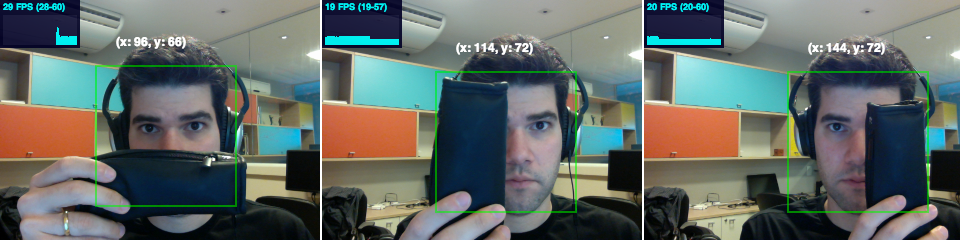
\includegraphics[width=\linewidth]{../chapters/evaluation/viola_occlusion.png}
  \end{figure}
\end{frame}

\subsection{Markerless tracking algorithm}

\begin{frame}{Examples}
  \begin{figure}[!htb]
    \centering
    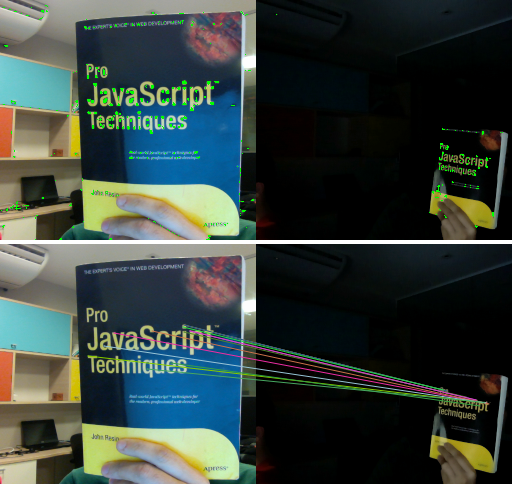
\includegraphics[width=140pt]{../chapters/evaluation/keypoints_fast_brief.png}
  \end{figure}
\end{frame}

\begin{frame}{Performance}
  \begin{figure}[!htb]
    \centering
      \begin{tikzpicture}[scale = 0.8]
      \begin{axis}[
          enlarge x limits=0.03,
          minor tick num=1,
          xlabel=Time (seconds),
          ylabel=Frames]

          \addplot[wblue,mark=x] coordinates {
          (0,25)
          (5,5)
          (10,4)
          (15,4)
          (20,4)
          (25,5)
          (30,4)
          (35,5)
          (40,4)
          (45,5)
          (50,4)
          (55,4)
          (60,4)
          (65,4)
          (70,5)
          (75,5)
          (80,5)
          (85,5)
          (90,4)
          (95,5)
          (100,4)
          (105,5)
          (110,4)
          (115,4)
          (120,5)
          (125,4)
          (130,4)
          (135,4)
          (140,5)
          (145,5)
          (150,4)
          (155,5)
          (160,4)
          (165,5)
          (170,4)
          (175,5)
          (180,4)
          (185,5)
          (190,5)
          (195,4)
          (200,4)
          (205,5)
          (210,5)
          (215,4)
          (220,5)
          (225,5)
          (230,5)
          (235,4)
          (240,5)
          (245,4)
          (250,4)
          (255,4)
          (260,5)
          (265,5)
          (270,5)
          (275,5)
          (280,5)
          (285,4)
          (290,4)
          (295,5)
          (300,4)
          (305,4)
          (310,4)
          (315,4)
          (320,4)
          (325,4)
          (330,5)
          (335,4)
          (340,4)
          (345,5)
          (350,5)
          (355,5)
          (360,4)
          (365,4)
          (370,5)
          (375,4)
          (380,5)
          (385,4)
          (390,4)
          (395,4)
          (400,4)
          (405,5)
          (410,4)
          (415,5)
          (420,5)
          (425,5)
          (430,4)
          (435,5)
          (440,5)
          (445,4)
          (450,4)
          (455,5)
          (460,5)
          (465,4)
          (470,5)
          (475,5)
          (480,4)
          (485,4)
          (490,5)
          (495,4)
          (500,5)
          (505,4)
          (510,4)
          (515,5)
          (520,4)
          (525,4)
          (530,5)
          (535,4)
          (540,5)
          (545,5)
          (550,5)
          (555,4)
          (560,4)
          (565,4)
          (570,5)
          (575,5)
          (580,4)
          (585,5)
          (590,5)
          (595,5)
          (600,4)
          (605,5)
          (610,4)
          (615,4)
          (620,4)
          (625,5)
          (630,5)
          (635,5)
          (640,4)
          (645,4)
          (650,4)
          (655,4)
          (660,5)
          (665,4)
          (670,5)
          (675,5)
          (680,4)
          (685,4)
          (690,4)
          (695,4)
          (700,5)
          (705,4)
          (710,4)
          (715,5)
          (720,4)
          (725,5)
          (730,4)
          (735,5)
          (740,5)
          (745,5)
          (750,5)
          (755,5)
          (760,5)
          (765,5)
          (770,5)
          (775,5)
          (780,5)
          (785,4)
          (790,4)
          (795,5)
          (800,5)
          (805,5)
          (810,5)
          (815,4)
          (820,5)
          (825,4)
          (830,4)
          (835,4)
          (840,4)
          (845,4)
          (850,5)
          (855,4)
          (860,4)
          (865,4)
          (870,5)
          (875,4)
          (880,5)
          (885,4)
          (890,5)
          (895,4)
          (900,5)
          (905,5)
          (910,4)
          (915,5)
          (920,5)
          (925,4)
          (930,4)
          (935,5)
          (940,5)
          (945,4)
          (950,4)
          (955,5)
          (960,4)
          (965,5)
          (970,4)
          (975,5)
          (980,4)
          (985,4)
          (990,4)
          (995,4)
          (1000,4)
           };

           \draw [red] ({rel axis cs:0,0}|-{axis cs:15,25}) -- ({rel axis cs:1,0}|-{axis cs:15,25}) node [pos=0.0, above] {};
      \end{axis}
      \end{tikzpicture}
  \end{figure}
\end{frame}

\begin{frame}{Oclusion robustness}
  \begin{figure}[!htb]
    \centering
    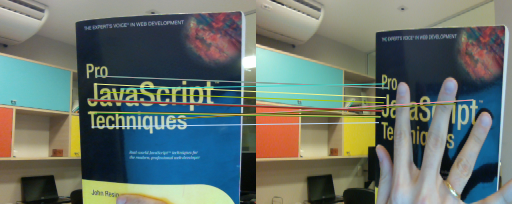
\includegraphics[width=\linewidth]{../chapters/evaluation/keypoints_occlusion.png}
  \end{figure}
\end{frame}
% % -----------------------------------------------------------------------------
\section{Conclusions}

\begin{frame}{Benefits of a JavaScript tracking solution}
  \small\addtolength{\tabcolsep}{-4pt}
  \begin{table}[!htb]
    \centering % here
    \begin{tabular}{|c|c|c|c|}
        \hline
        & OSAKit & \textit{tracking.js} + color & \textit{tracking.js} + face \\
        \hline
        Avg frame rate & 25 FPS & 30 FPS & 25 FPS\\
        \hline
        Avg file size & 22 MB & 8 KB & 187 KB\\
        \hline
        Avg load time (256 Kbps) & 11 min & 0.25 seconds & 5 seconds\\
        \hline
    \end{tabular}
  \end{table}
\end{frame}

\begin{frame}{Contributions}
  \begin{itemize}
    \item A tracking library for the web called \textit{tracking.js}
    \item Optimizations for existing techniques in order to run in real-time on the web
    \item Pioneered a library that brings state-of-the-art techniques for computer vision to the web
    \item Academic material about web browser concepts
  \end{itemize}
\end{frame}

\begin{frame}{Future work}
  \begin{itemize}
    \item Publication detailing web browser concepts
    \item Publication comparing client-side JavaScript based tracking with client-side plugin-based and server-side solutions
    \item Double Exponential Smoothing technique
    \item Perspective-$n$-Point problem (P$n$P) calculation
    \item Image processing layer capable of transformations and filters
  \end{itemize}
\end{frame}

\begin{frame}{Website}
  \begin{figure}[!htb]
    \centering
    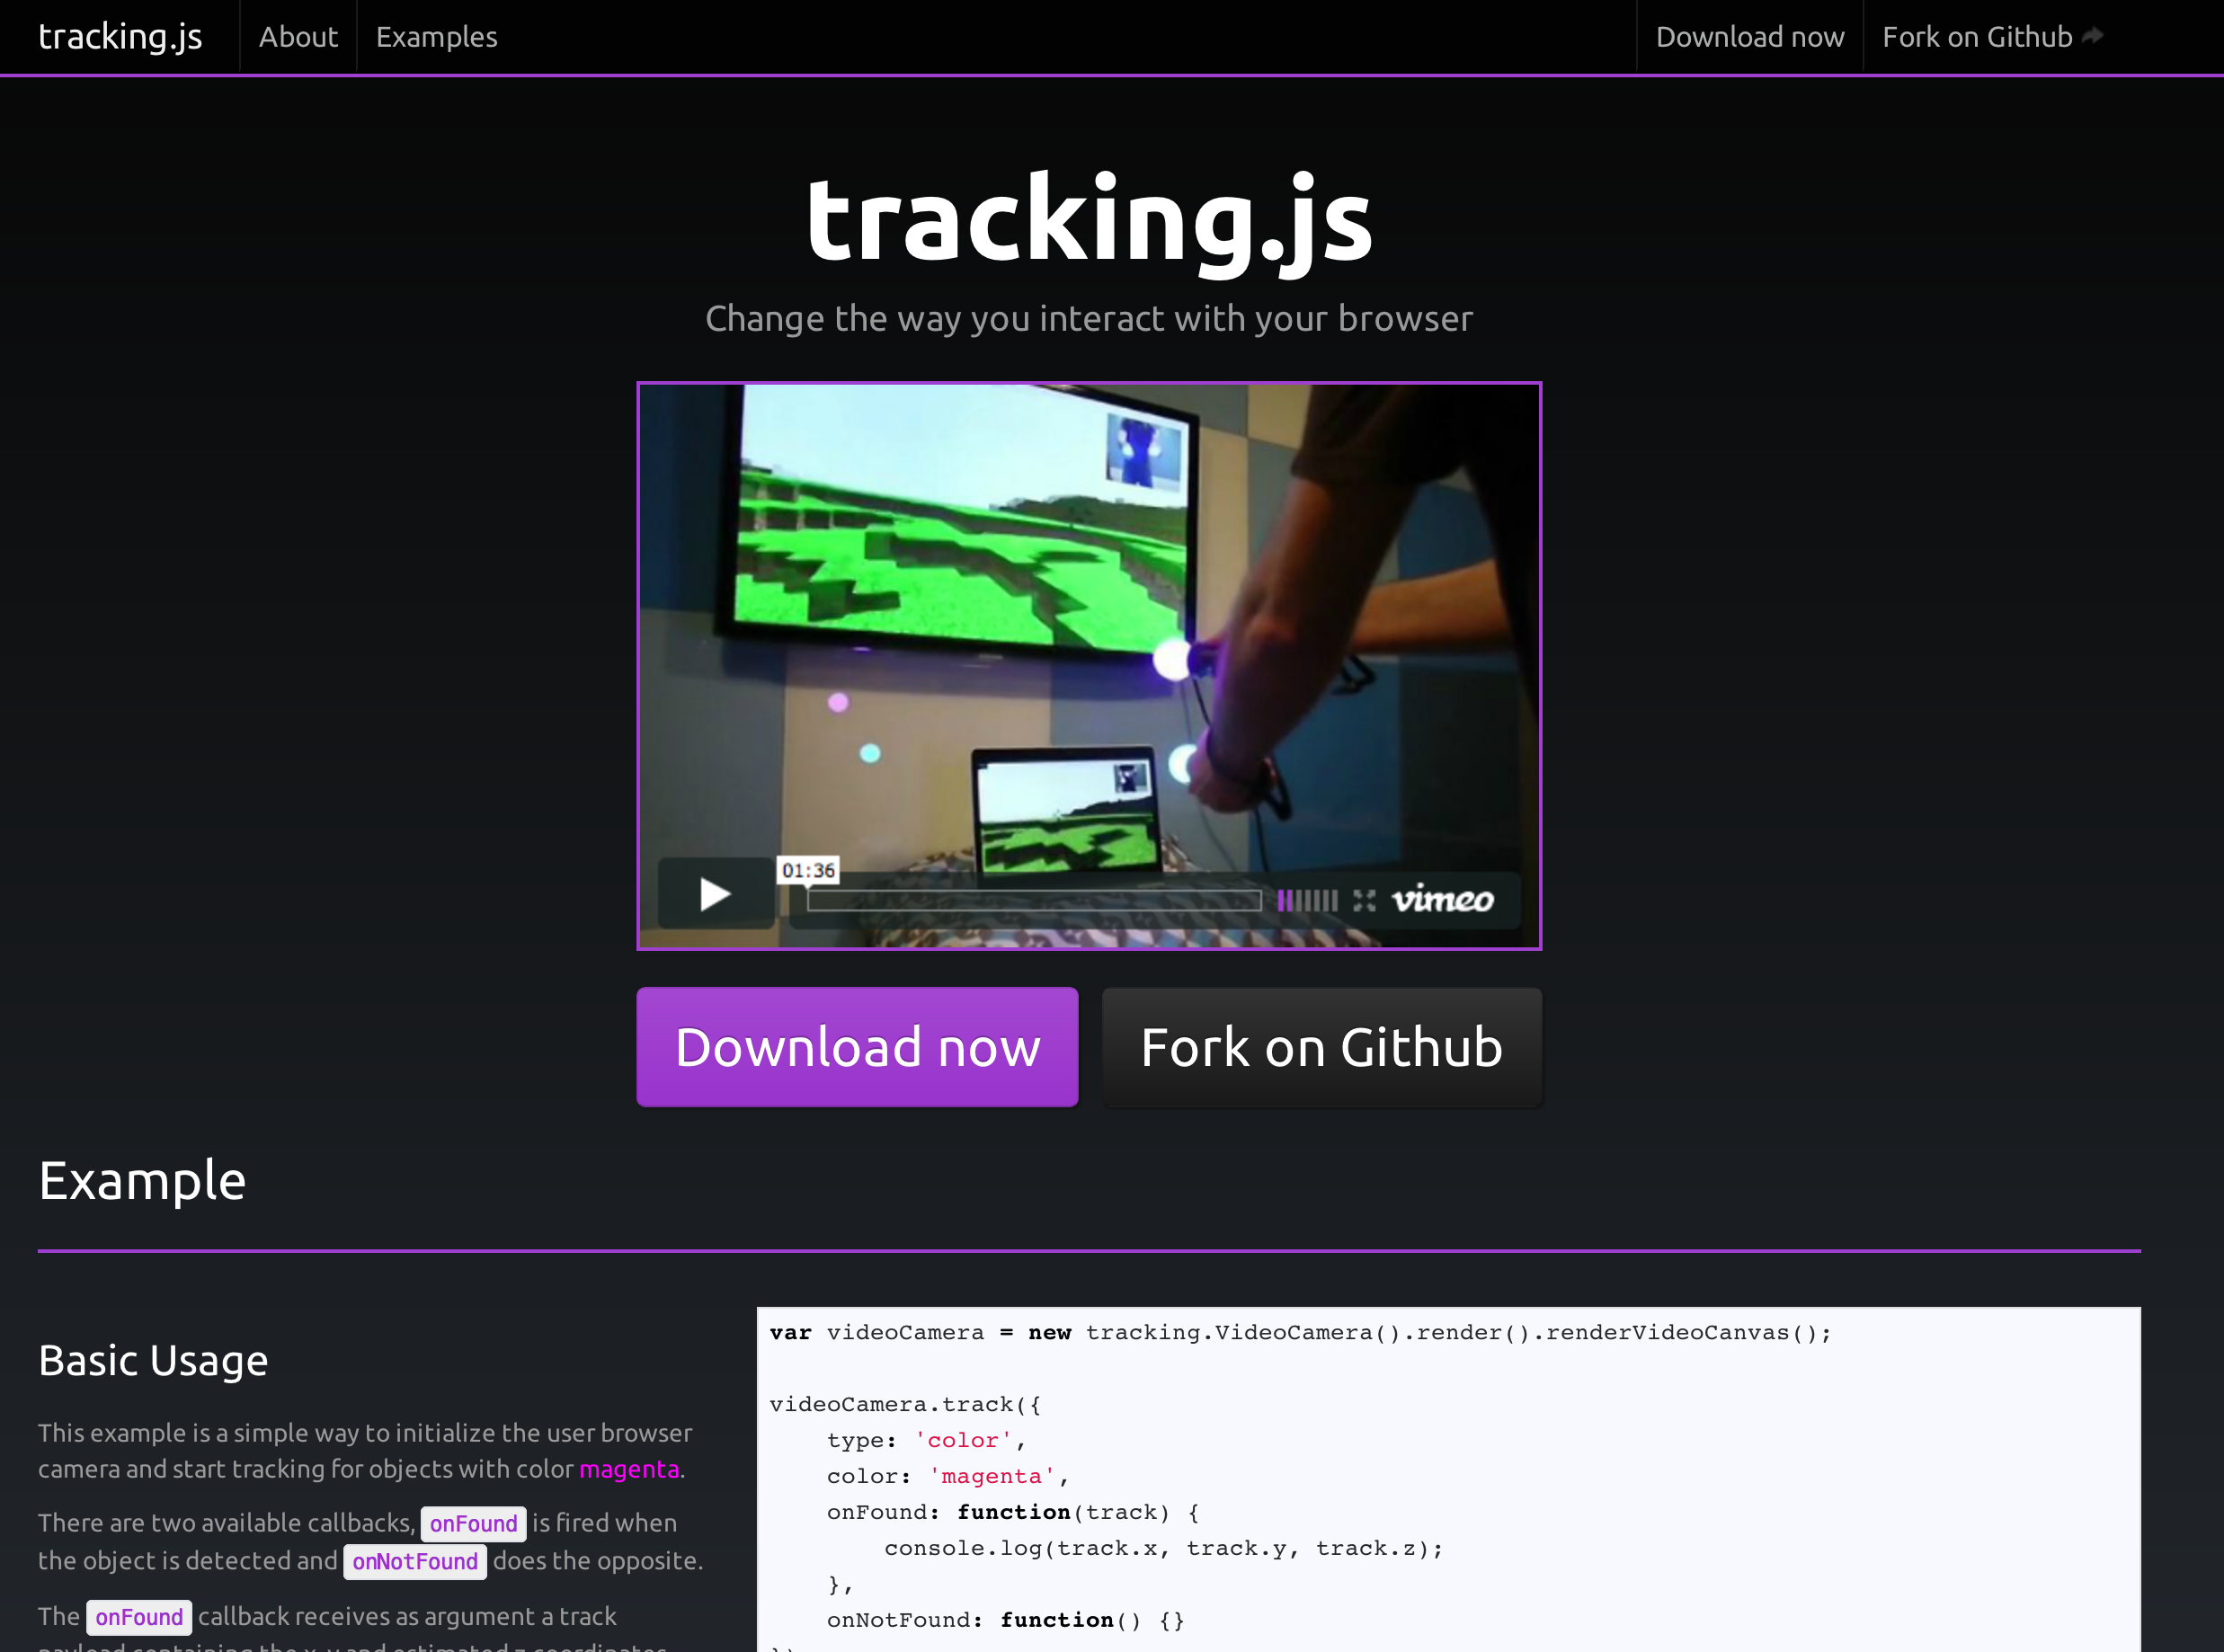
\includegraphics[width=180pt]{site.png}
    \caption{\url{http://trackingjs.com}}
  \end{figure}
\end{frame}

\begin{frame}{Popularity}
  \begin{figure}[!htb]
    \centering
    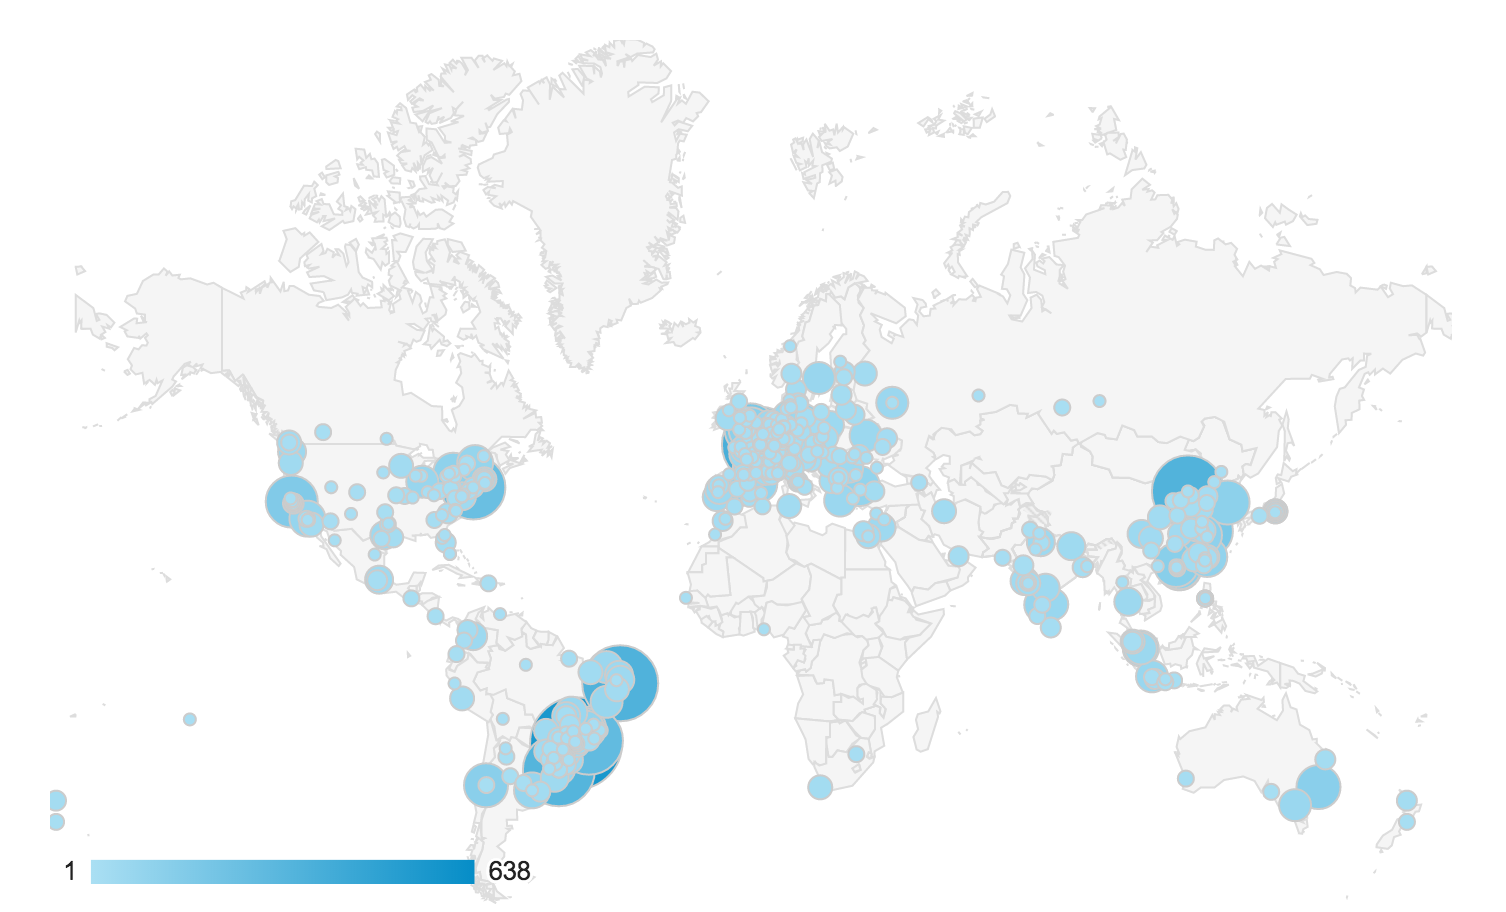
\includegraphics[width=260pt]{repercussion_site.png}
  \end{figure}
\end{frame}

\begin{frame}{Popularity}
  \begin{figure}[!htb]
    \centering
    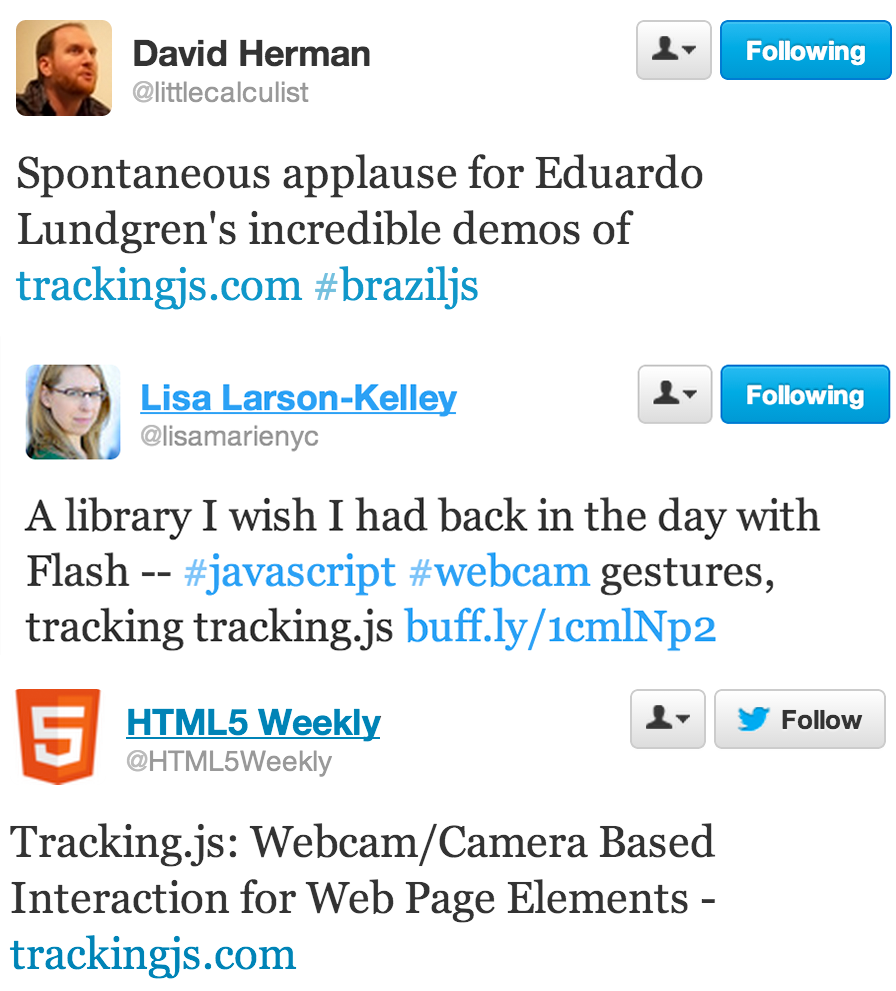
\includegraphics[width=140pt]{repercussion.png}
  \end{figure}
\end{frame}

\begin{frame}{Popularity}
  \begin{itemize}
    \item 445 tweets mentioning \textit{tracking.js}
    \item 31,258 website page views
    \item Project hosted on Mozilla Developer Network
    \item Talk presented on DevFest Brazil - Brazil, 2012
    \item Talk presented on W3C Conference - Brazil, 2012
    \item Talk presented on HTML5 Dev Conf - USA, 2013
    \item Talk accepted on JS.everywhere - USA, 2013
  \end{itemize}
\end{frame}

\begin{frame}{Thank you!}
\end{frame}
% -----------------------------------------------------------------------------
\end{document}
